\documentclass[11pt,final,onecolumn]{report}

\usepackage[utf8x]{inputenc}
\usepackage[british]{babel}
\usepackage{verbatim,boxedminipage}
%\usepackage[a4paper, inner=0.5cm, outer=0.5cm, top=1cm,
%bottom=1.5cm, bindingoffset=1cm]{geometry}
\usepackage{amsmath}
\usepackage{amssymb, latexsym}
\usepackage{longtable}
\usepackage[table]{xcolor}
\usepackage{textcomp} 
\usepackage{stmaryrd}
\usepackage{graphicx}
\usepackage{enumitem}
\usepackage{yfonts}
\usepackage{algpseudocode}
\usepackage{algorithm}
\usepackage{hyperref}
\usepackage{MnSymbol}

\setlist[enumerate]{label*=\arabic*.}
\newtheorem{theorem}{Theorem}[section]
\newtheorem{example}{Example}[section]
\newtheorem{definition}{Definition}[section]
\newtheorem{proposition}{Proposition}[section]
\newtheorem{notation}{Notation}[section]

\renewcommand{\algorithmicrequire}{\textbf{Input:}}
\renewcommand{\algorithmicensure}{\textbf{Output:}}

\newcommand\umltablespacing{3cm}
\newcommand\dltablespacing{4.5cm}
\newcommand\owlspacing{-1mm}  

\title{UML Class Diagram to OWL and SROIQ Reference}
\author{Henriette Harmse}
\date{}

\pdfinfo{%
  /Title    (UML Class Diagram to OWL and SROIQ Reference)
  /Author   (Henriette Harmse)
  /Creator  ()
  /Producer ()
  /Subject  ()
  /Keywords (OWL, Manchester Syntax, UML class diagrams)
}

\begin{document}
    \maketitle
    
    \begin{longtable}{|>{\scriptsize}c|>{\scriptsize}l|>{\scriptsize}l|}
    KILLED & LINE!!!! \kill
    \hiderowcolors
%     \caption{UML class diagram to OWL 2 and $\mathcal{SROIQ}^{(\mathcal{D})}$ Reference}\\
    \hline
    \textbf{UML class diagram feature} & $\mathcal{SROIQ}^{(\mathcal{D})}$ & \textbf{OWL 2}
    \endhead
    \hline  
    \begin{minipage}{\umltablespacing}    
      \centering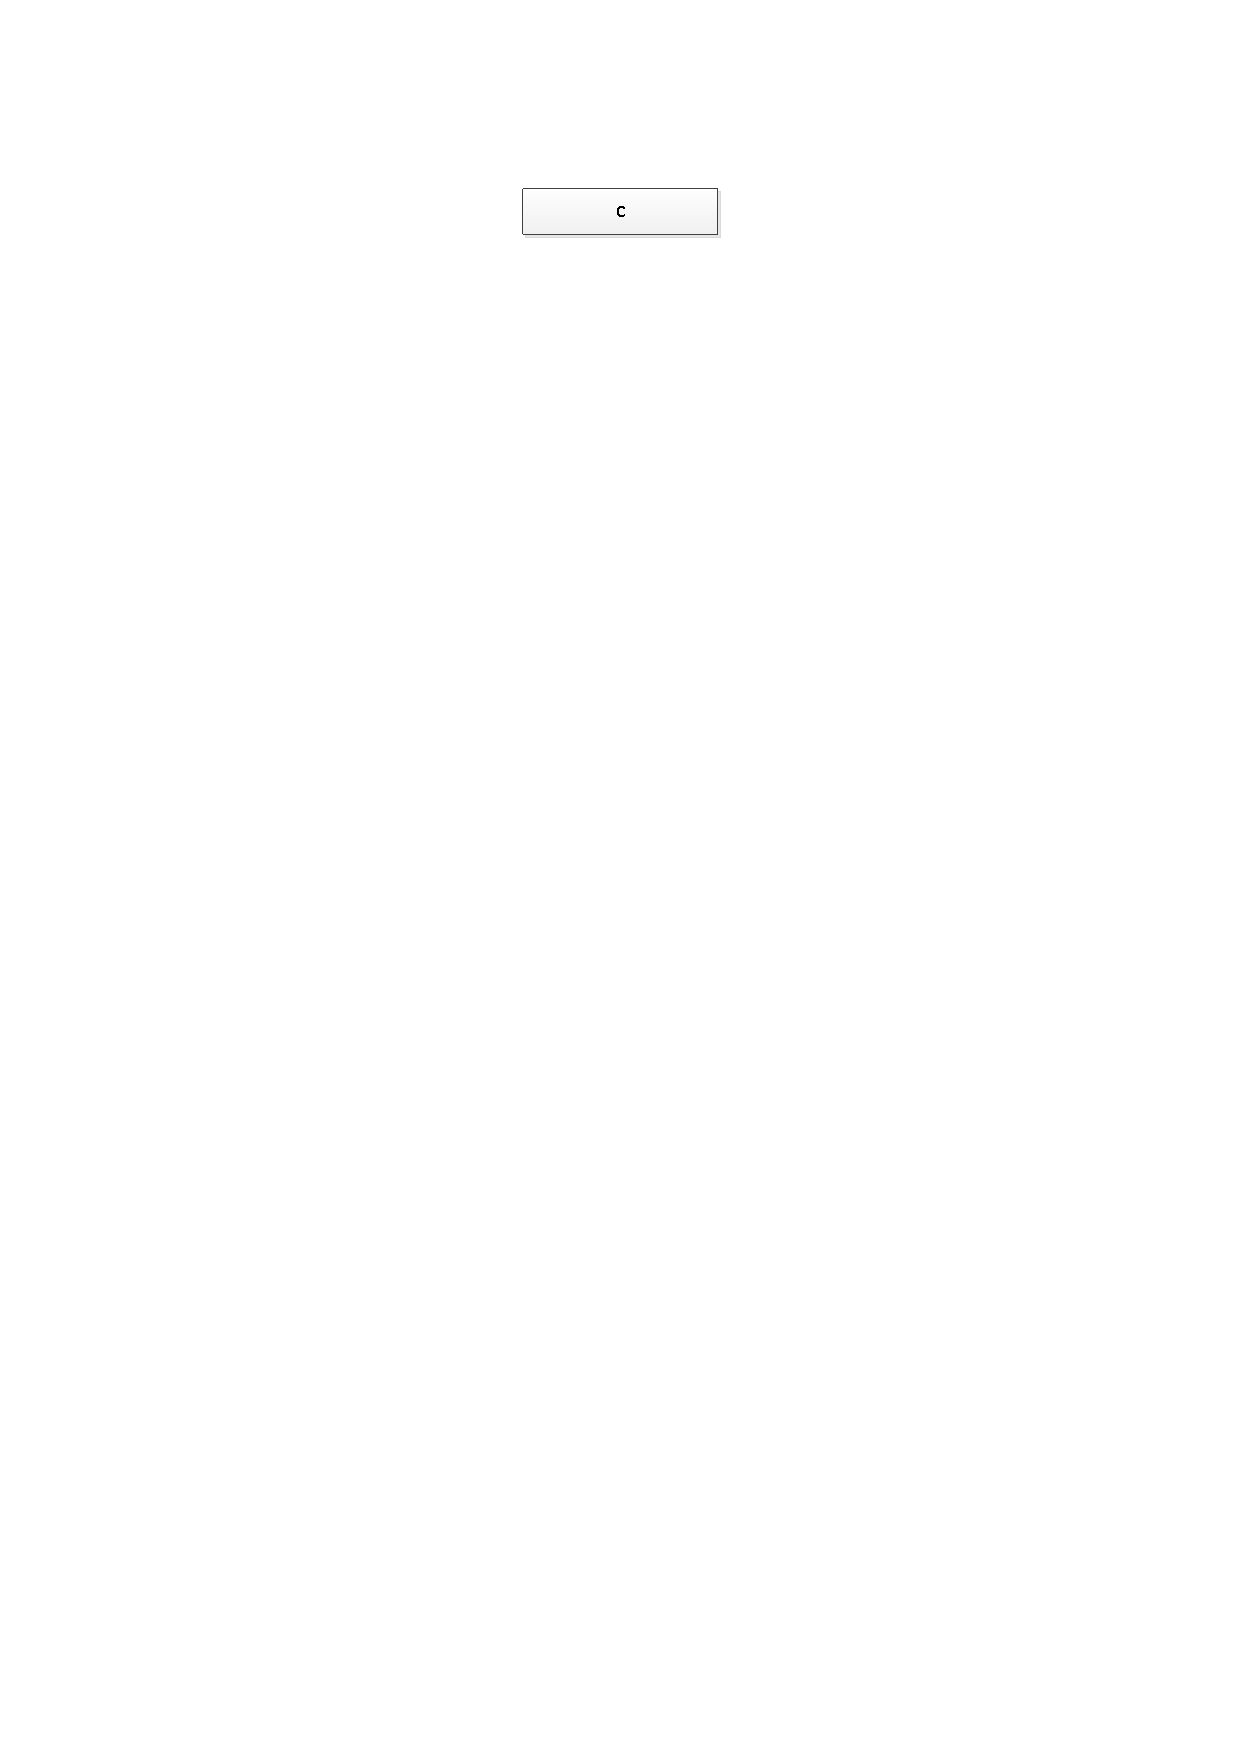
\includegraphics[trim = 85mm 257mm 70mm 22mm, clip, scale=0.75]{./diagrams/chapter5/Class}
       Class \texttt{C}       
       \vspace{2mm}
    \end{minipage}
    &
    \begin{minipage}{\dltablespacing}
       $\begin{aligned}  
       \\
	  C
         \end{aligned}$       
    \end{minipage}
    &
      $\begin{aligned}
	  &\texttt{}\\
	  &\texttt{Class: C}
     \end{aligned}$
    \\\hline
    \begin{minipage}{\umltablespacing}  
      \centering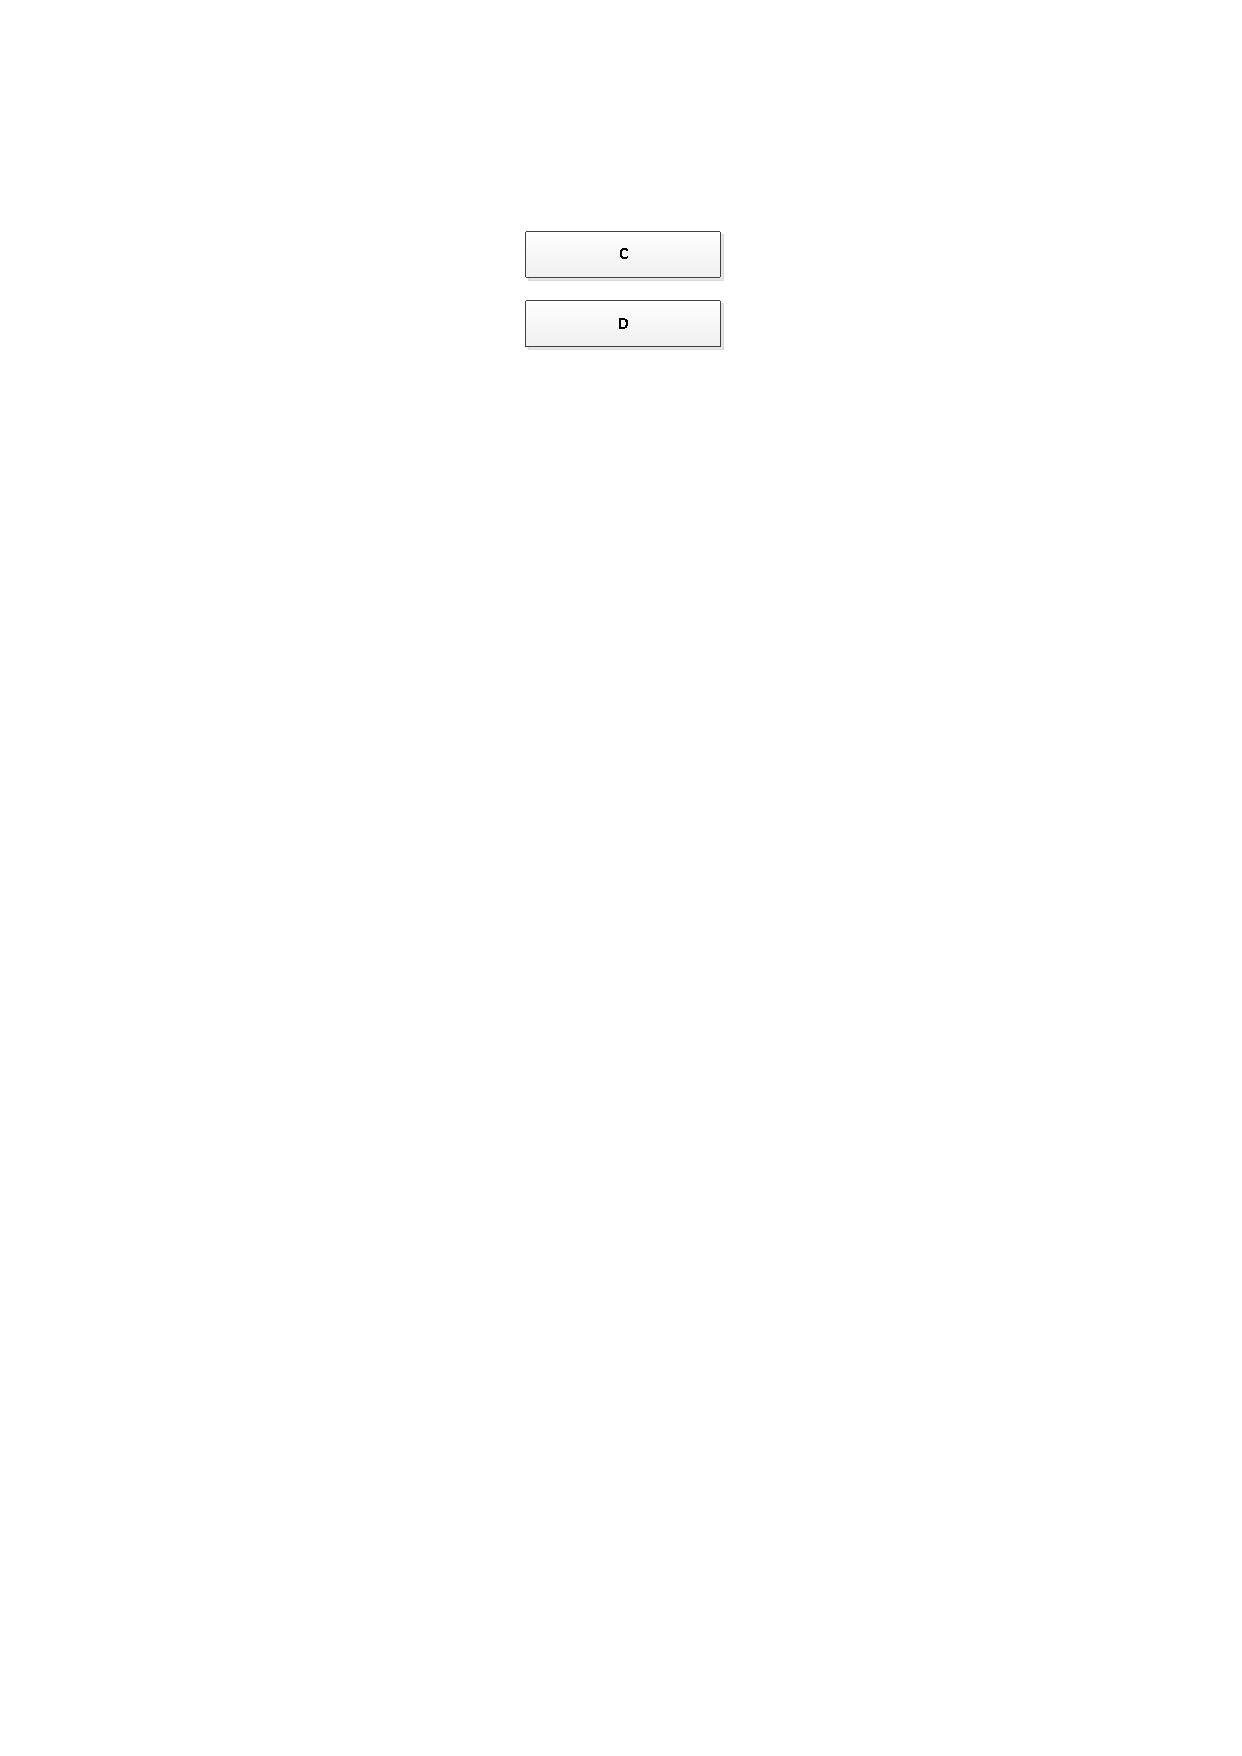
\includegraphics[trim = 85mm 238mm 70mm 28mm, clip, scale=0.75]{./diagrams/chapter5/DisjointClasses}
     Classes \texttt{C} and \texttt{D}
     \vspace{2mm}
    \end{minipage}
    &
    \begin{minipage}{\dltablespacing}
       $\begin{aligned}   
	  C \sqsubseteq \neg D
       \end{aligned}$       
    \end{minipage}
    &
      $\begin{aligned}
	  &\texttt{}\\
	  &\texttt{Class: C}\\[\owlspacing]
	  &\texttt{Class: D}\\[\owlspacing]
	  &\texttt{\hspace*{0.2cm}DisjointWith: C}
     \end{aligned}$
    \\\hline
    \begin{minipage}{\umltablespacing}    
      \centering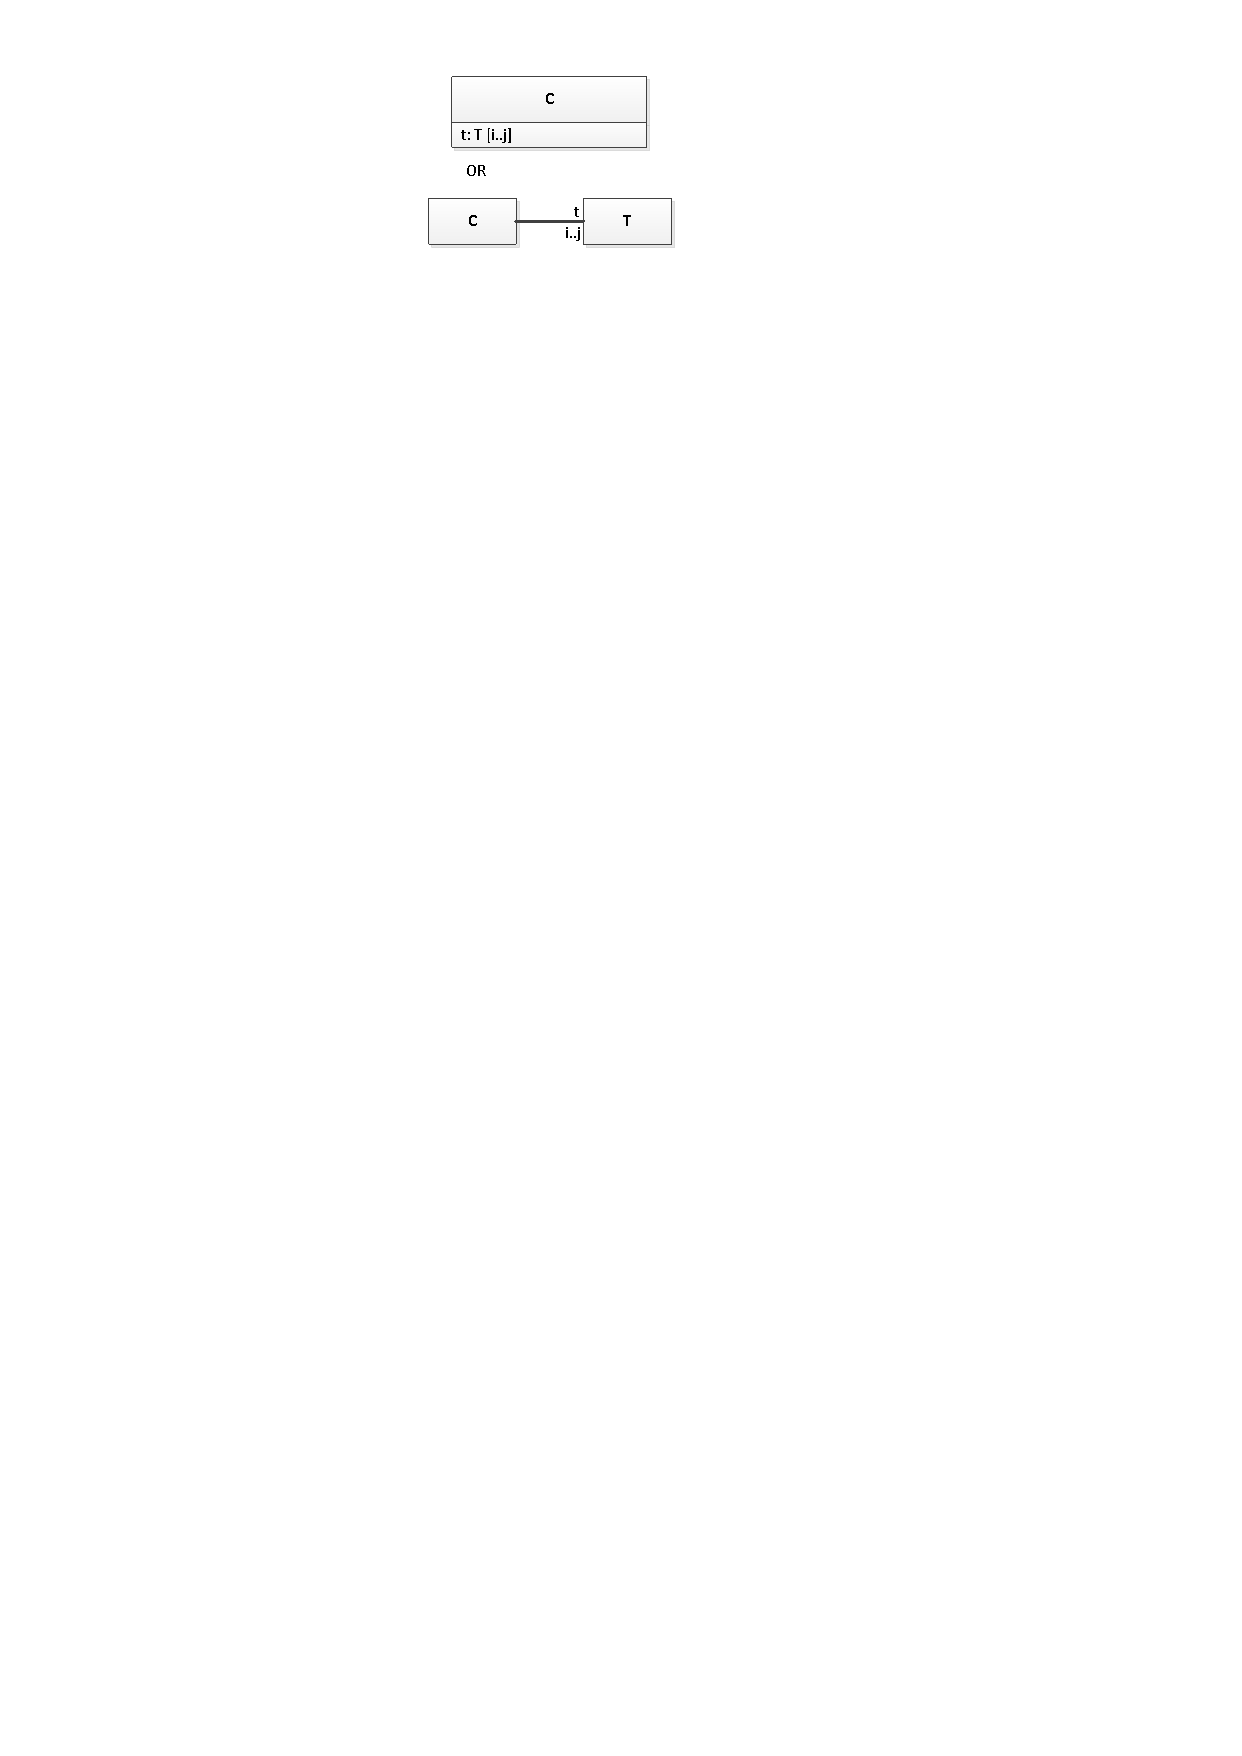
\includegraphics[trim = 72mm 250mm 92mm 4mm, clip, scale=0.75]{./diagrams/chapter5/Attribute} 
     Attribute \texttt{t} of type \texttt{T} with multiplicity \texttt{[i..j]} \\OR\\ Association end \texttt{t} of type \texttt{T} with multiplicity \texttt{[i..j]}
     \vspace{2mm}
    \end{minipage}
    &
    \begin{minipage}{\dltablespacing}
       $\begin{aligned}
	  &\exists t.\top \sqsubseteq \hspace*{2pt} C \\
          &\exists t^-.\top \sqsubseteq \hspace*{2pt} T \\
	  &C \sqsubseteq \hspace*{2pt} (\geq i \hspace*{2pt} t.\top) \hspace*{2pt} \sqcap \hspace*{2pt} (\leq j \hspace*{2pt} t.\top)
       \end{aligned}$      
    \end{minipage}
    &
      $\begin{aligned}
         &\texttt{}\\
	 &\texttt{Class: C}\\[\owlspacing]
	 &\texttt{\hspace*{2mm}SubClassOf:} \\[\owlspacing]
	 &\texttt{\hspace*{2mm}(t min i Thing) and}\\[\owlspacing]
	 &\texttt{\hspace*{4mm}(t max j Thing)} \\[\owlspacing]         
         &\texttt{Class: T}\\[\owlspacing]
         &\texttt{ObjectProperty: t} \\[\owlspacing]
         &\texttt{\hspace*{2mm}Domain: C} \\[\owlspacing]
         &\texttt{\hspace*{2mm}Range: T} \\[\owlspacing]
	 &\texttt{}\\
     \end{aligned}$
    \\\hline
    \begin{minipage}{\umltablespacing}    
      \centering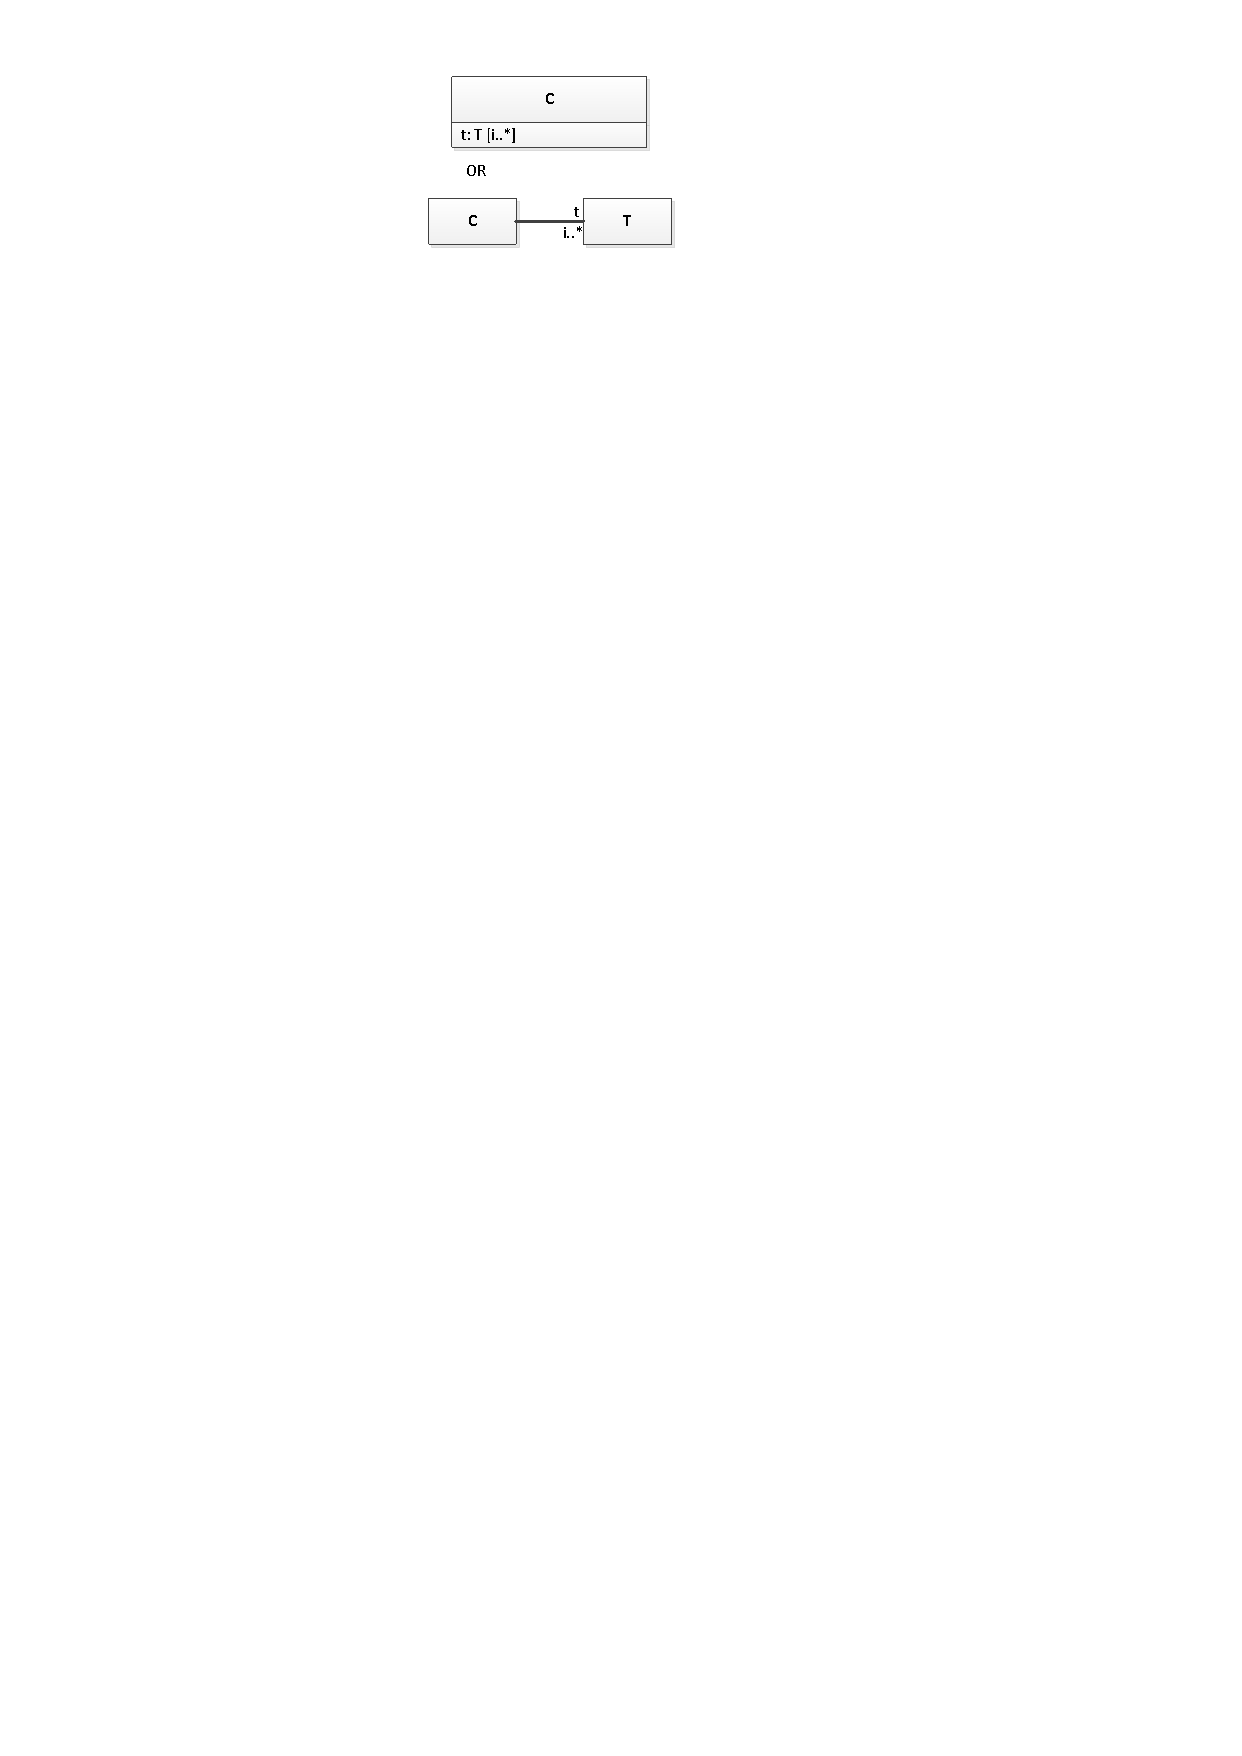
\includegraphics[trim = 72mm 250mm 92mm 4mm, clip, scale=0.75]{./diagrams/chapter5/AttributeMultiplicity_j2infinity} 
     Attribute \texttt{t} of type \texttt{T} with multiplicity \texttt{[i..*]} \\OR\\ Association end \texttt{t} of type \texttt{T} with multiplicity \texttt{[i..*]}
     \vspace{2mm}
    \end{minipage}
    &
    \begin{minipage}{\dltablespacing}
       $\begin{aligned}
	  &\exists t.\top \sqsubseteq \hspace*{2pt} C \\
          &\exists t^-.\top \sqsubseteq \hspace*{2pt} T \\
	  &C \sqsubseteq \hspace*{2pt} (\geq i \hspace*{2pt} t.\top) \hspace*{2pt}
       \end{aligned}$      
    \end{minipage}
    &
      $\begin{aligned}
         &\texttt{}\\
	 &\texttt{Class: C}\\[\owlspacing]
	 &\texttt{\hspace*{2mm}SubClassOf:} \\[\owlspacing]
	 &\texttt{\hspace*{2mm}(t min i Thing)}\\[\owlspacing]         
         &\texttt{Class: T}\\[\owlspacing]
         &\texttt{ObjectProperty: t} \\[\owlspacing]
         &\texttt{\hspace*{2mm}Domain: C} \\[\owlspacing]
         &\texttt{\hspace*{2mm}Range: T} \\[\owlspacing]
	 &\texttt{}\\
     \end{aligned}$  
    \\\hline
    \begin{minipage}{\umltablespacing}    
      \centering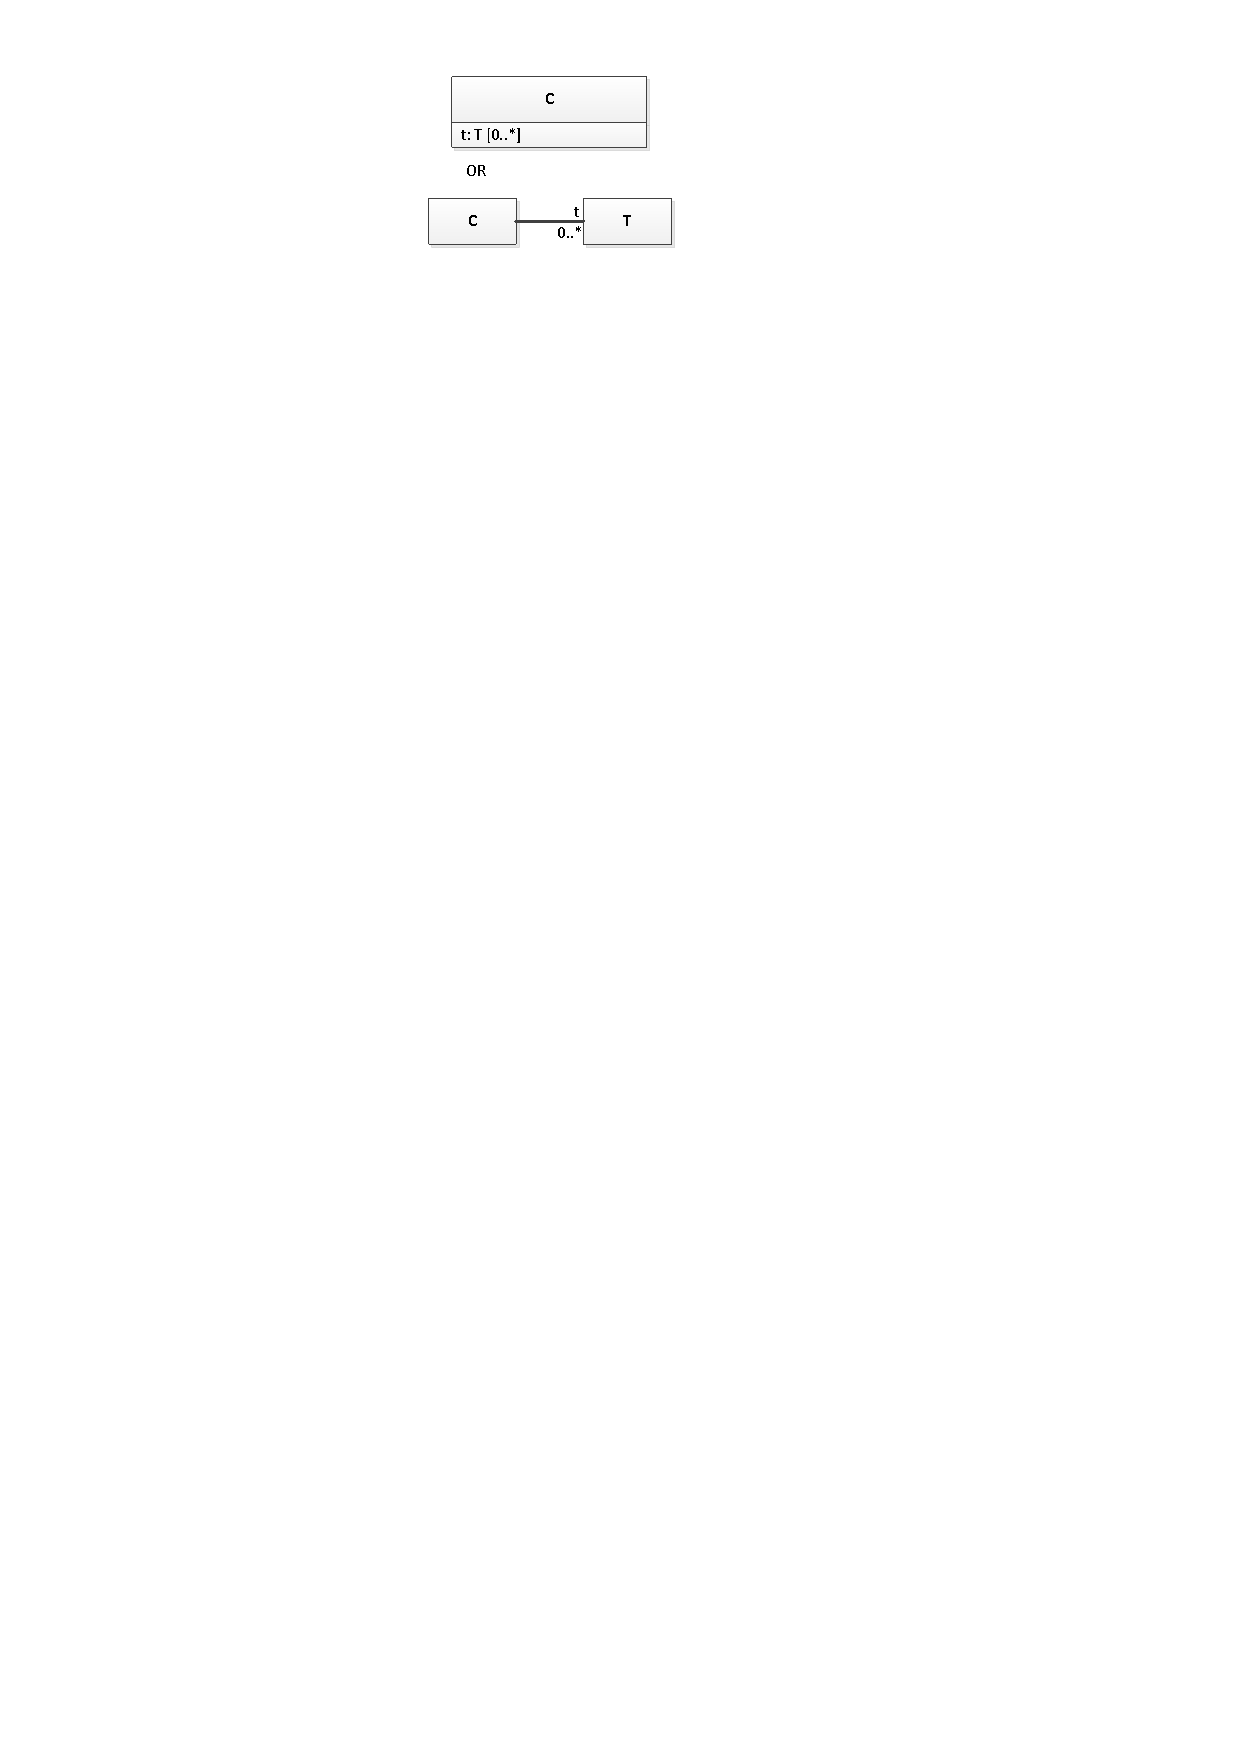
\includegraphics[trim = 72mm 250mm 92mm 4mm, clip, scale=0.75]{./diagrams/chapter5/AttributeMultiplicity_02infinity} 
     Attribute \texttt{t} of type \texttt{T} with multiplicity \texttt{[0..*]} \\OR\\ Association end \texttt{t} of type \texttt{T} with multiplicity \texttt{[0..*]}
     \vspace{2mm}
    \end{minipage}
    &
    \begin{minipage}{\dltablespacing}
       $\begin{aligned}
	  &\exists t.\top \sqsubseteq \hspace*{2pt} C \\
          &\exists t^-.\top \sqsubseteq \hspace*{2pt} T
       \end{aligned}$      
    \end{minipage}
    &
       $\begin{aligned}
         &\texttt{}\\
         &\texttt{Class: C}\\[\owlspacing]
         &\texttt{Class: T}\\[\owlspacing]
         &\texttt{ObjectProperty: t} \\[\owlspacing]
         &\texttt{\hspace*{2mm}Domain: C} \\[\owlspacing]
         &\texttt{\hspace*{2mm}Range: T} \\[\owlspacing]
	 &\texttt{}\\
     \end{aligned}$  
    \\\hline
    \begin{minipage}{\umltablespacing}    
      \centering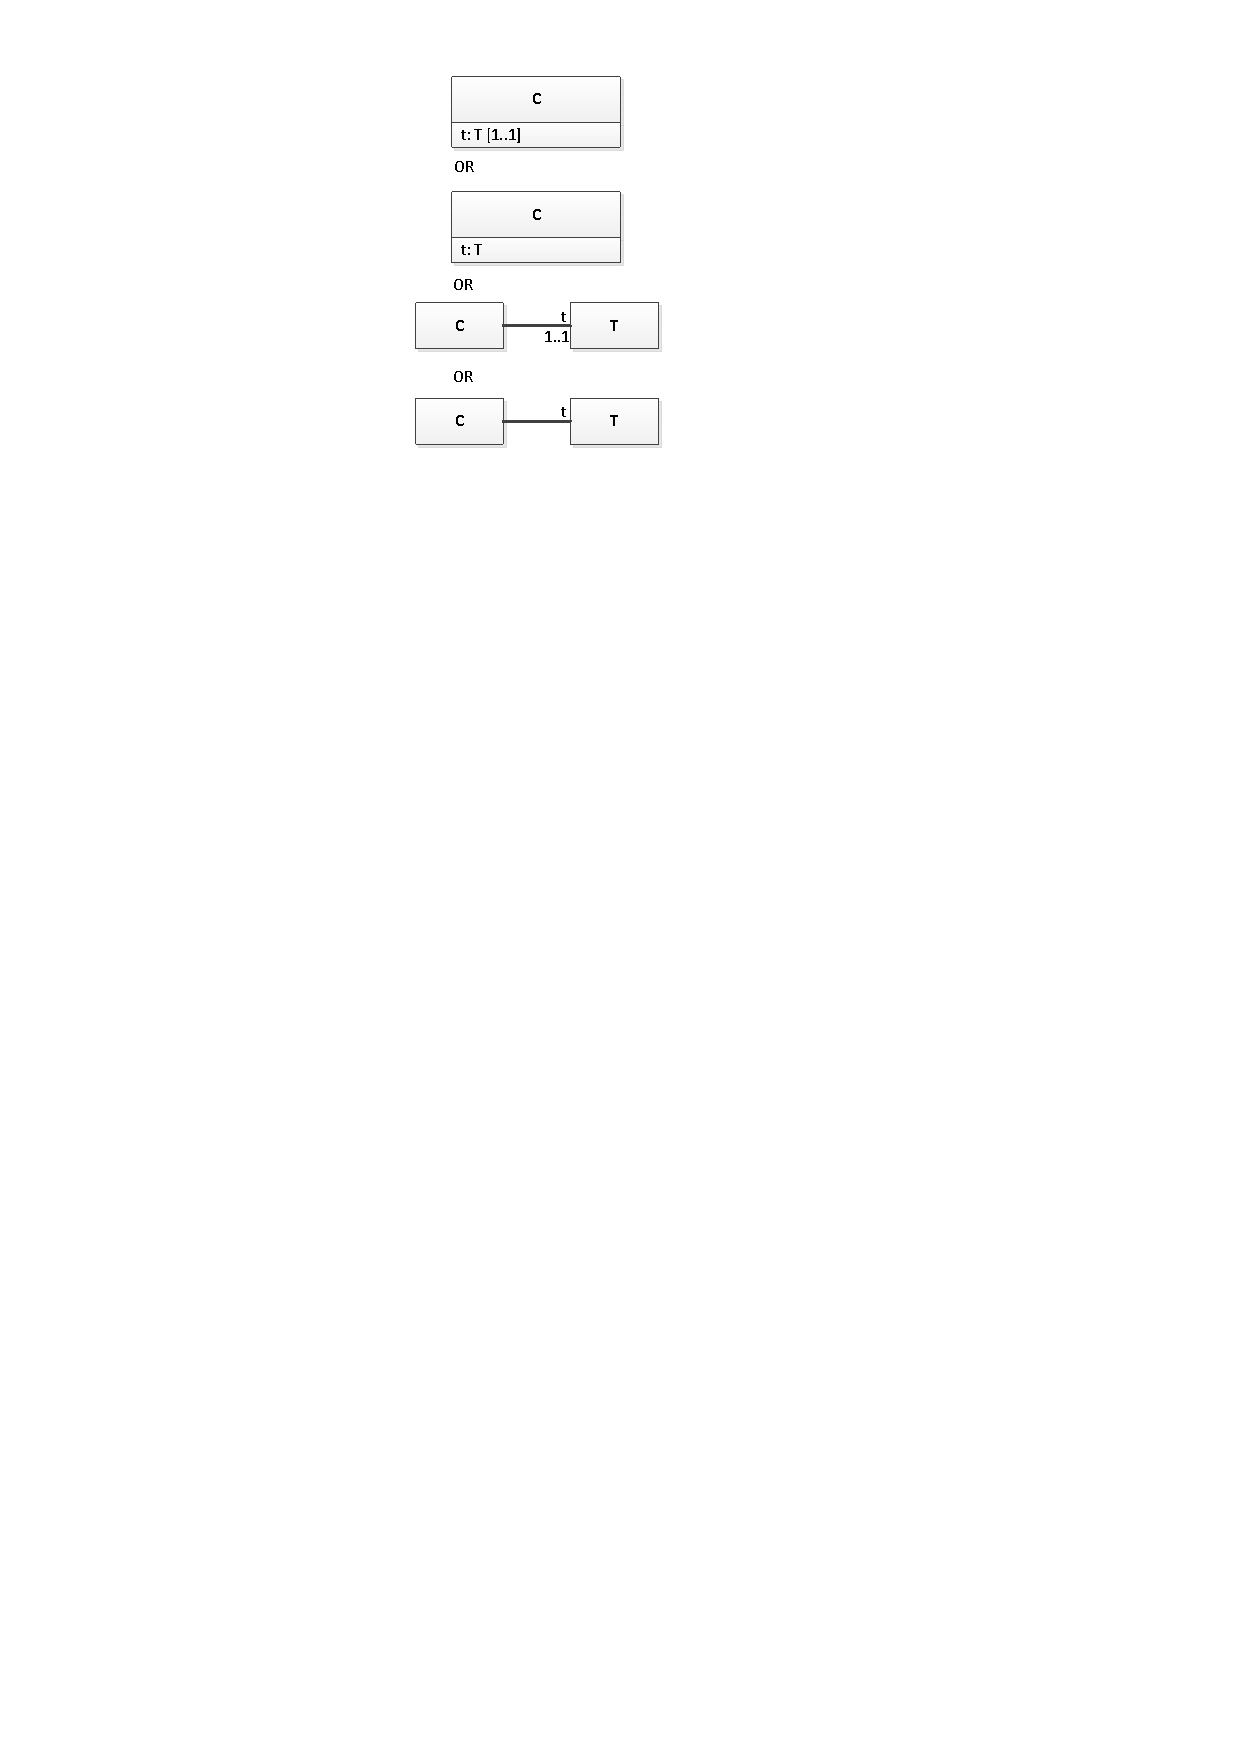
\includegraphics[trim = 70mm 220mm 92mm 4mm, clip, scale=0.75]{./diagrams/chapter5/AttributeMultiplicity1} 
     Attribute \texttt{t} of type \texttt{T} with multiplicity \texttt{[1..1]} \\OR\\ Association end \texttt{t} of type \texttt{T} with multiplicity \texttt{[1..1]}
     \vspace{2mm}
    \end{minipage}
    &
    \begin{minipage}{\dltablespacing}
       $\begin{aligned}
       	 &\exists t.\top \sqsubseteq \hspace*{2pt} C \\
         &\exists t^-.\top \sqsubseteq \hspace*{2pt} T \\
	 &C \sqsubseteq \exists t.\top \sqcap (\leq 1 \hspace*{2pt} t. \top)
       \end{aligned}$      
    \end{minipage}
    &
      $\begin{aligned}
	&\texttt{Class: C}\\[\owlspacing]
   	&\texttt{\hspace*{2mm}SubClassOf:}\\[\owlspacing]
   	&\texttt{\hspace*{4mm}t exactly 1 Thing}\\[\owlspacing]      
	&\texttt{Class: T}
     \end{aligned}$
    \\\hline  
    \begin{minipage}{\umltablespacing}
      \centering\hspace*{-4mm}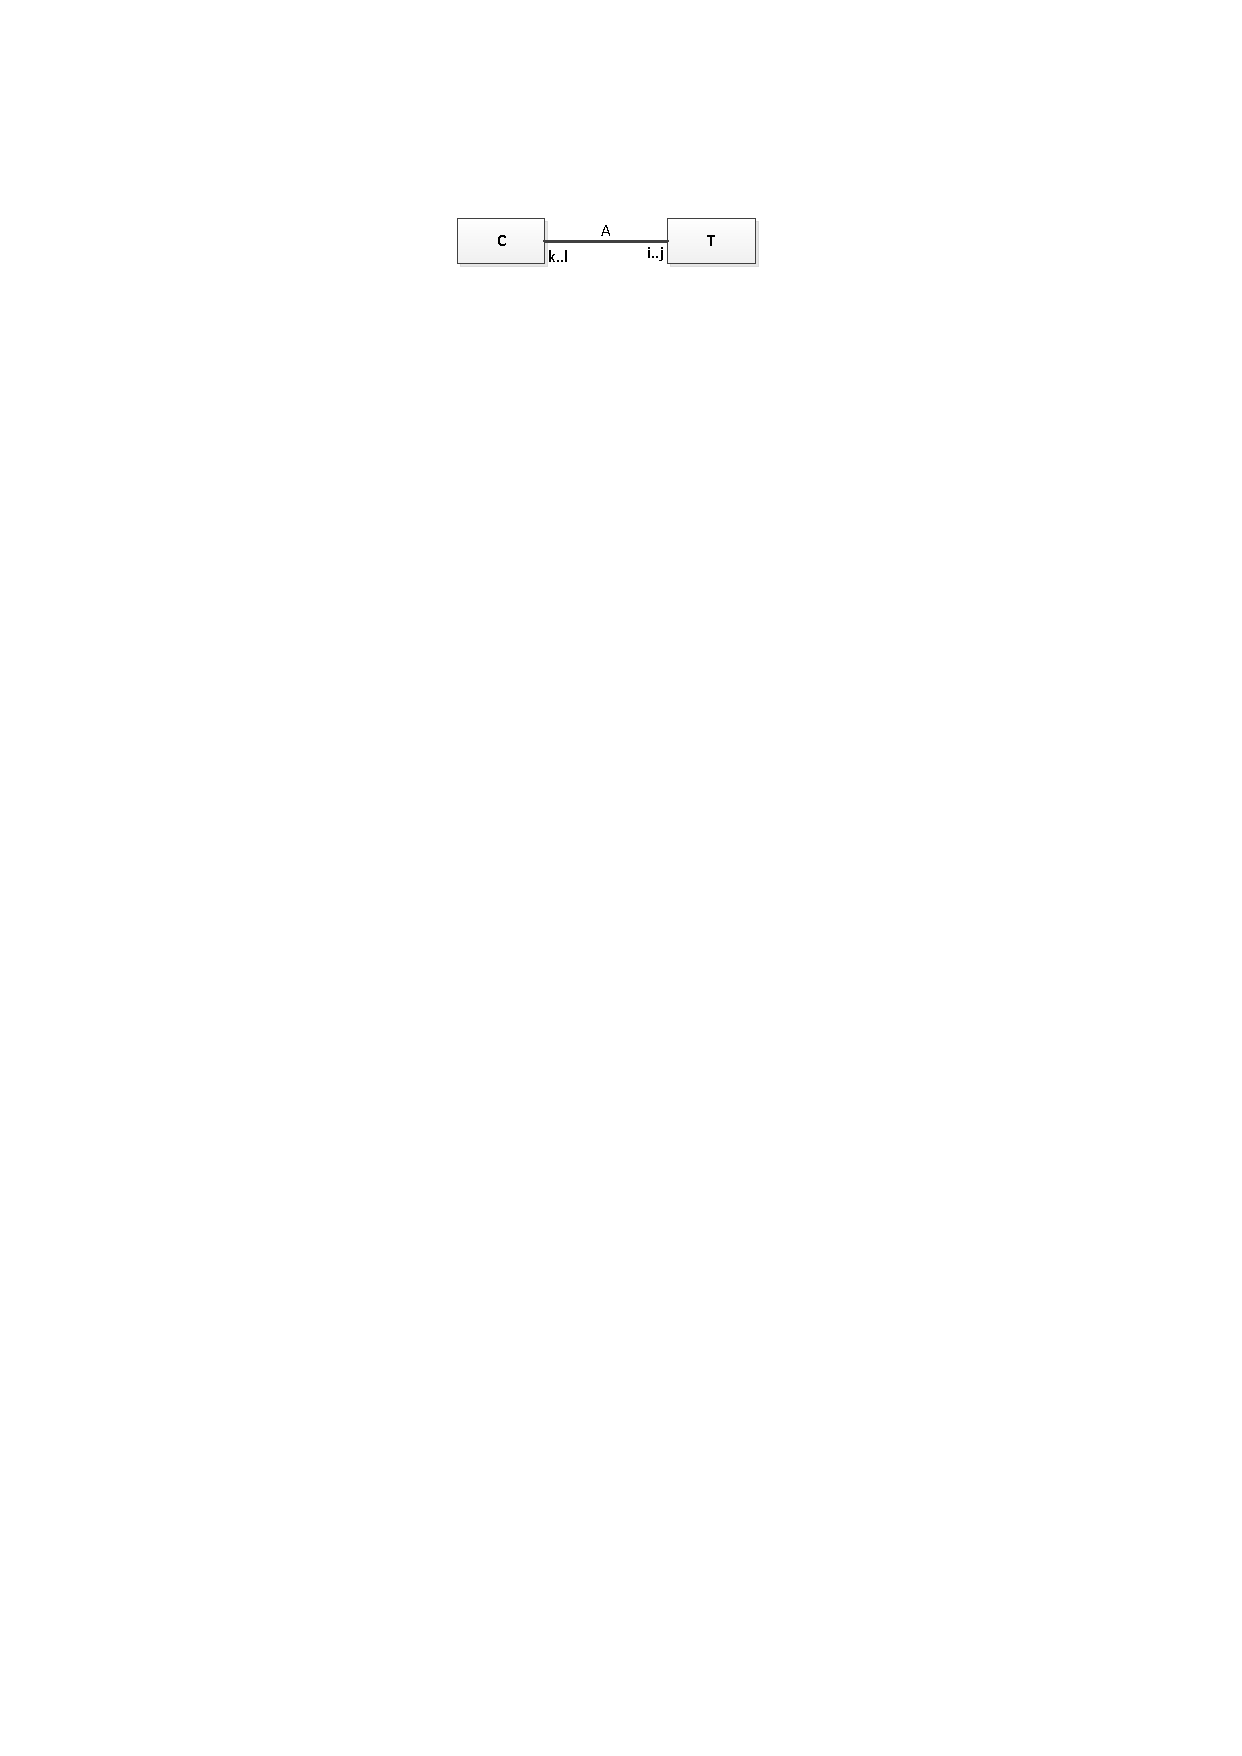
\includegraphics[trim = 77mm 245mm 74mm 25mm, clip, scale=0.75]{./diagrams/chapter5/Association}
      Association \texttt{A} exists between classes \texttt{C} and \texttt{T}
      %Classes \texttt{C1} and \texttt{C2} are disjoint and specialize class \texttt{C} without covering class it 
     \vspace{2mm}
    \end{minipage}
    &
    \begin{minipage}{\dltablespacing}
       $\begin{aligned}   
	  &\exists a.\top \sqsubseteq \hspace*{2pt} C \\
          &\exists a^-.\top \sqsubseteq \hspace*{2pt} T \\
          &C \sqsubseteq (\geq i \hspace*{2pt} a.\top) \sqcap (\leq j \hspace*{2pt} a.\top)\\
          &T \sqsubseteq (\geq k \hspace*{2pt} a^-.\top) \sqcap (\leq l \hspace*{2pt} a^-.\top)\\	  
         \end{aligned}$      
    \end{minipage}
    &
      $\begin{aligned}
        \\
   	&\texttt{ObjectProperty: a}\\[\owlspacing]
    	&\texttt{\hspace*{0.20cm}Domain: C} \\[\owlspacing]
    	&\texttt{\hspace*{0.20cm}Range: T}\\[\owlspacing]
    	&\texttt{ObjectProperty: a\_inv}\\[\owlspacing]
    	&\texttt{\hspace*{0.20cm}InverseOf: a} \\
   	&\texttt{Class: C}\\[\owlspacing]
   	&\texttt{\hspace*{0.20cm}SubClassOf:}\\[\owlspacing]
   	&\texttt{\hspace*{0.40cm}(a min i Thing) and}\\[\owlspacing]
   	&\texttt{\hspace*{0.40cm}(a max j Thing)}\\
   	&\texttt{Class: T}\\[\owlspacing]
   	&\texttt{\hspace*{0.20cm}SubClassOf:}\\[\owlspacing]
   	&\texttt{\hspace*{0.40cm}(a\_inv min k Thing) and}\\[\owlspacing]
   	&\texttt{\hspace*{0.40cm}(a\_inv max l Thing)}\\
   	\\
     \end{aligned}$      
    \\\hline  
    \begin{minipage}{\umltablespacing}
      \centering\hspace*{-4mm}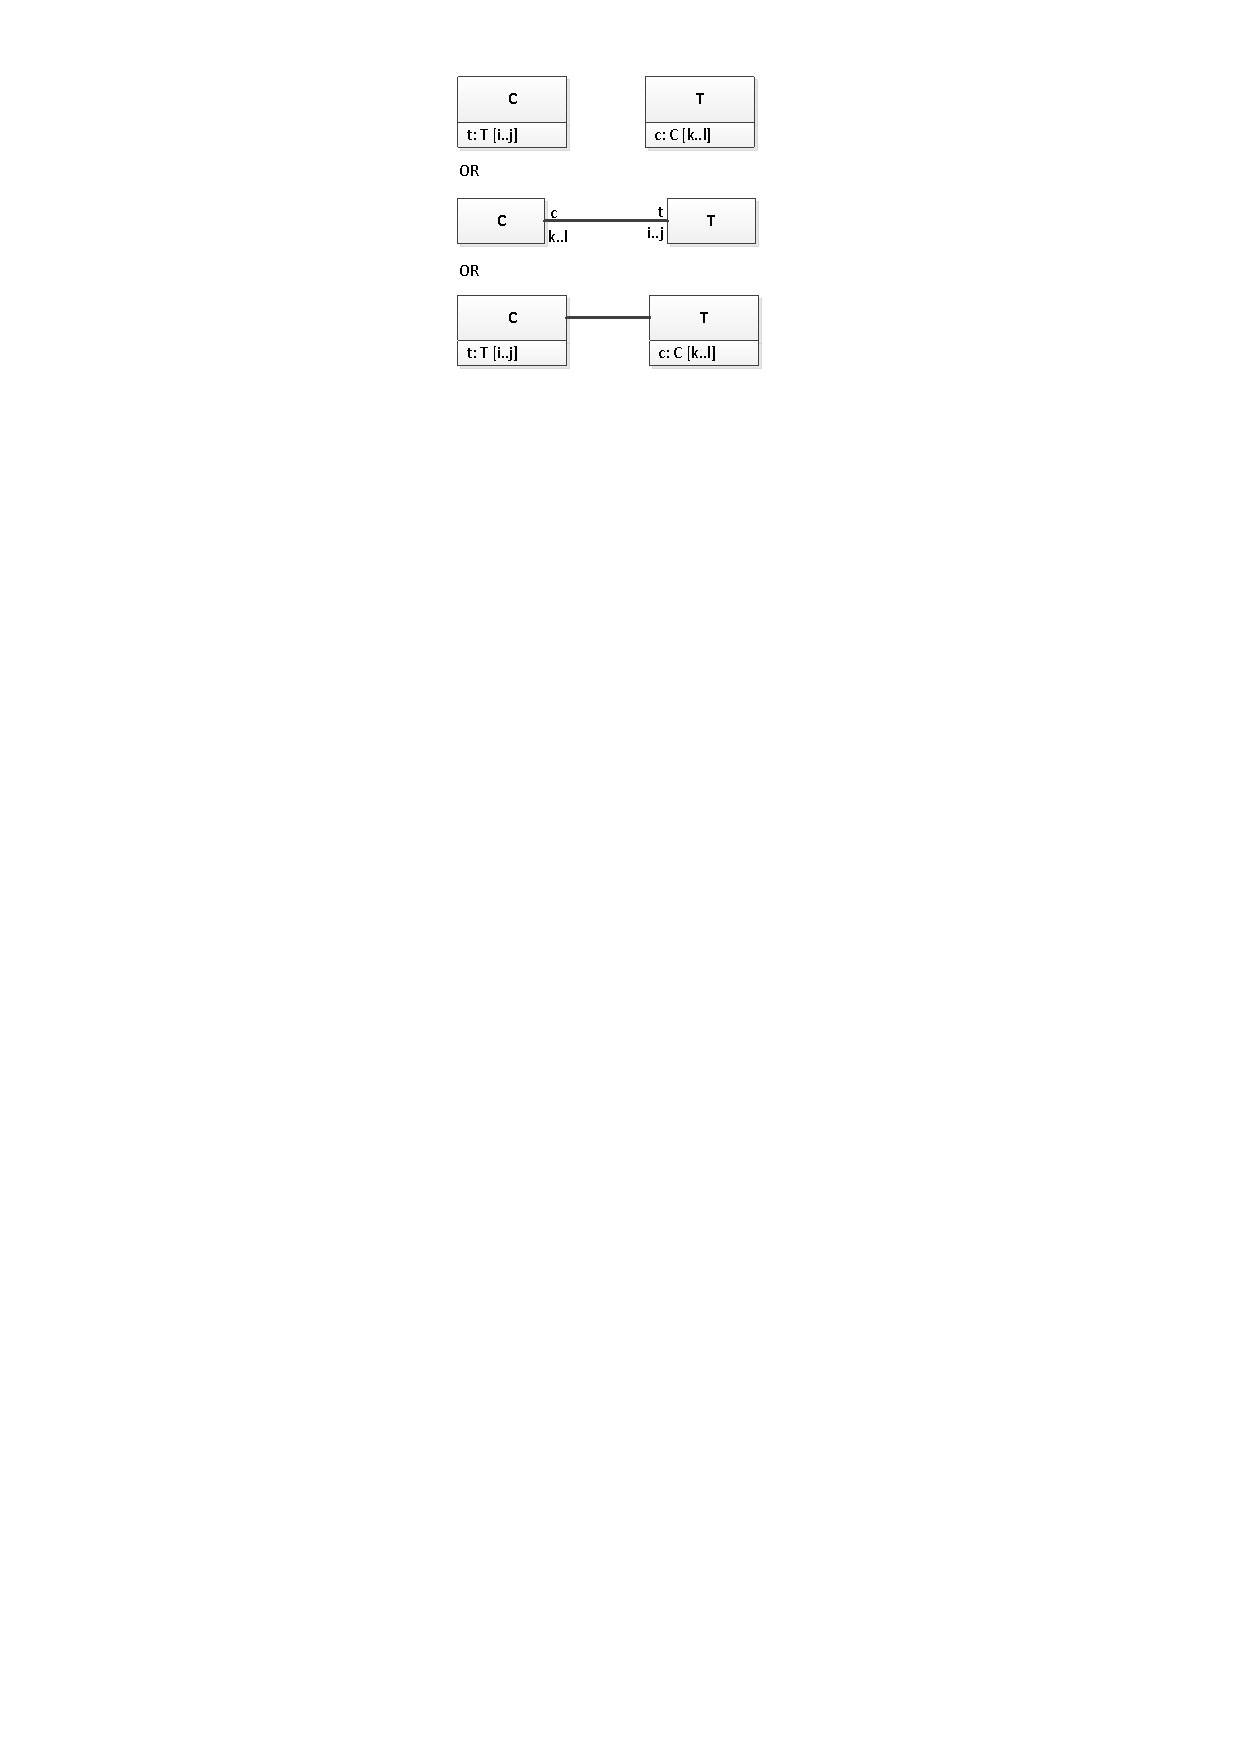
\includegraphics[trim = 77mm 230mm 74mm 5mm, clip, scale=0.75]{./diagrams/chapter5/AssociationEnds}
      Attribute \texttt{t} of type \texttt{T} with multiplicity \texttt{[i..j]} belongs to class \texttt{C}
      and attribute \texttt{c} of type \texttt{C} with multiplicity \texttt{[k..l]} belongs to class \texttt{T}
      \\OR\\
      Association end \texttt{t} with multiplicity \texttt{[i..j]} is associated with class \texttt{C} and asociation end \texttt{c} with multiplicity \texttt{[k..l]} is associated with class \texttt{T}
      \\OR\\
      Line notation is used to make explicit that attributes \texttt{t} and \texttt{c} are also association ends
      %Classes \texttt{C1} and \texttt{C2} are disjoint and specialize class \texttt{C} without covering class it 
     \vspace{2mm}
    \end{minipage}
    &
    \begin{minipage}{\dltablespacing}
       $\begin{aligned}    
	  &\exists t.\top \sqsubseteq \hspace*{2pt} C \\
          &\exists t^-.\top \sqsubseteq \hspace*{2pt} T \\
	  &C \sqsubseteq \hspace*{2pt} (\geq i \hspace*{2pt} t.\top) \hspace*{2pt} \sqcap \hspace*{2pt} (\leq j \hspace*{2pt} t.\top)\\
	  \\
	  &c \equiv t^-\\
	  &T \sqsubseteq \hspace*{2pt} (\geq k \hspace*{2pt} c.\top) \hspace*{2pt} \sqcap \hspace*{2pt} (\leq l \hspace*{2pt} c.\top)\\	  
         \end{aligned}$      
    \end{minipage}
    &
      $\begin{aligned}
         &\texttt{}\\
         &\texttt{ObjectProperty: t} \\[\owlspacing]
         &\texttt{\hspace*{2mm}Domain: C} \\[\owlspacing]
         &\texttt{\hspace*{2mm}Range: T} \\[\owlspacing]
	 &\texttt{Class: C}\\[\owlspacing]
	 &\texttt{\hspace*{2mm}SubClassOf:} \\[\owlspacing]
	 &\texttt{\hspace*{2mm}(t min i Thing) and}\\[\owlspacing]
	 &\texttt{\hspace*{4mm}(t max j Thing)} \\
         &\texttt{ObjectProperty: c} \\[\owlspacing]
         &\texttt{\hspace*{2mm}InverseOf: t}\\[\owlspacing]
	 &\texttt{Class: T}\\[\owlspacing]
	 &\texttt{\hspace*{2mm}SubClassOf:} \\[\owlspacing]
	 &\texttt{\hspace*{2mm}(c min k Thing) and}\\[\owlspacing]
	 &\texttt{\hspace*{4mm}(c max l Thing)} \\[\owlspacing]
   	\\
     \end{aligned}$    
    \\\hline
    \begin{minipage}{\umltablespacing}
      \centering\hspace*{-4mm}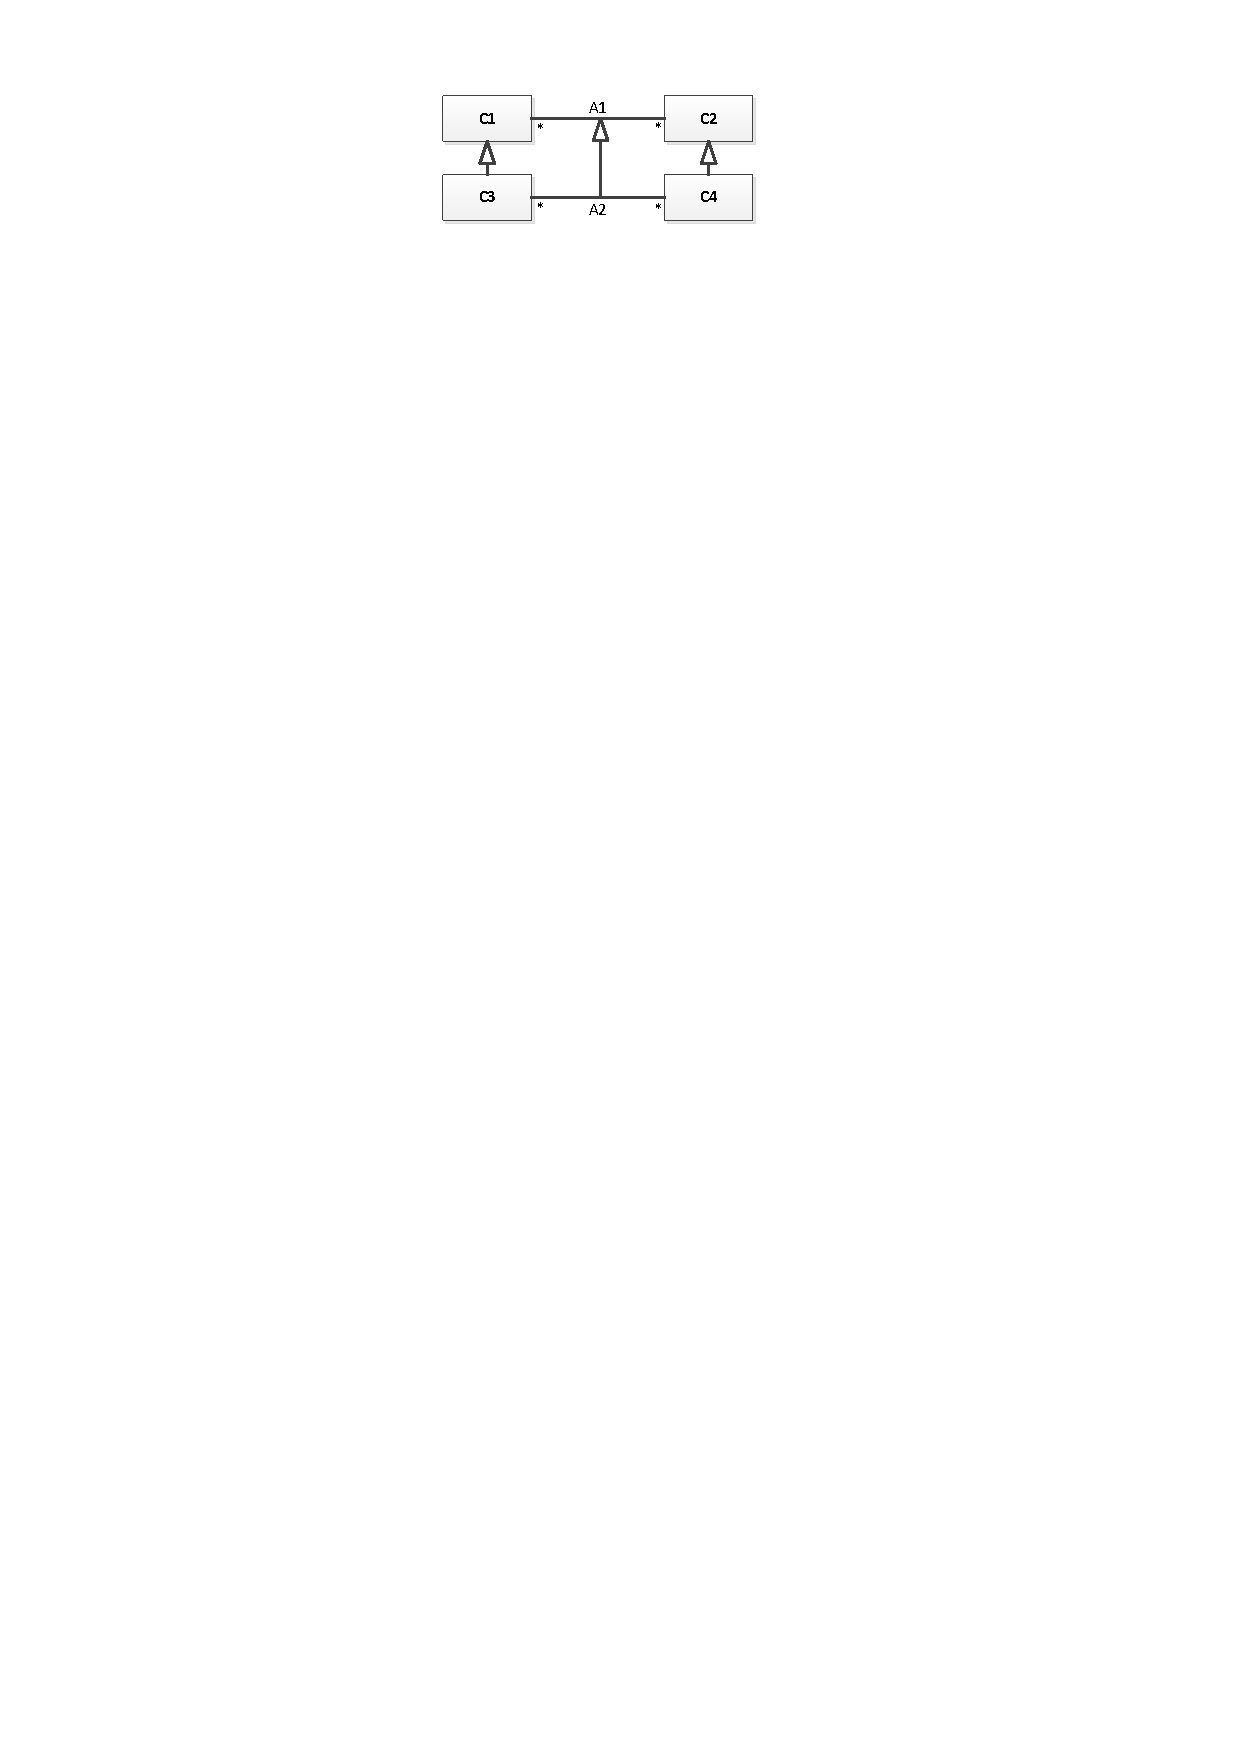
\includegraphics[trim = 75mm 255mm 72mm 5mm, clip, scale=0.75]{./diagrams/chapter5/AssociationSpecialization}
      Association \texttt{A2} specializes association \texttt{A1} 
     \vspace{2mm}
    \end{minipage}
    &
    \begin{minipage}{\dltablespacing}
       $\begin{aligned}    	  
          &\exists a_1.\top \sqsubseteq C_1\\ 
          &\exists a_1^-.\top \sqsubseteq C_2\\
          &\exists a_2.\top \sqsubseteq C_3\\ 
          &\exists a_2^-.\top \sqsubseteq C_4\\
          &a_2 \sqsubseteq a_1\\
         \end{aligned}$      
    \end{minipage}
    &
      $\begin{aligned}
        \\
        &\texttt{Class: C1}\\[\owlspacing]
        &\texttt{Class: C2}\\[\owlspacing]
        &\texttt{Class: C3}\\[\owlspacing]
        &\texttt{Class: C4}\\[\owlspacing]        
        &\texttt{ObjectProperty: a1}\\[\owlspacing]
        &\texttt{\hspace*{2mm}Domain: C1} \\[\owlspacing]
        &\texttt{\hspace*{2mm}Range: C2} \\[\owlspacing]
   	&\texttt{ObjectProperty: a2}\\[\owlspacing]
        &\texttt{\hspace*{2mm}Domain: C3} \\[\owlspacing]
        &\texttt{\hspace*{2mm}Range: C4} \\[\owlspacing]   	
    	&\texttt{\hspace*{2mm}SubPropertyOf: a1} \\
    	&\texttt{}\\
     \end{aligned}$
    \\\hline
    \begin{minipage}{\umltablespacing}
      \centering\hspace*{-6.3mm}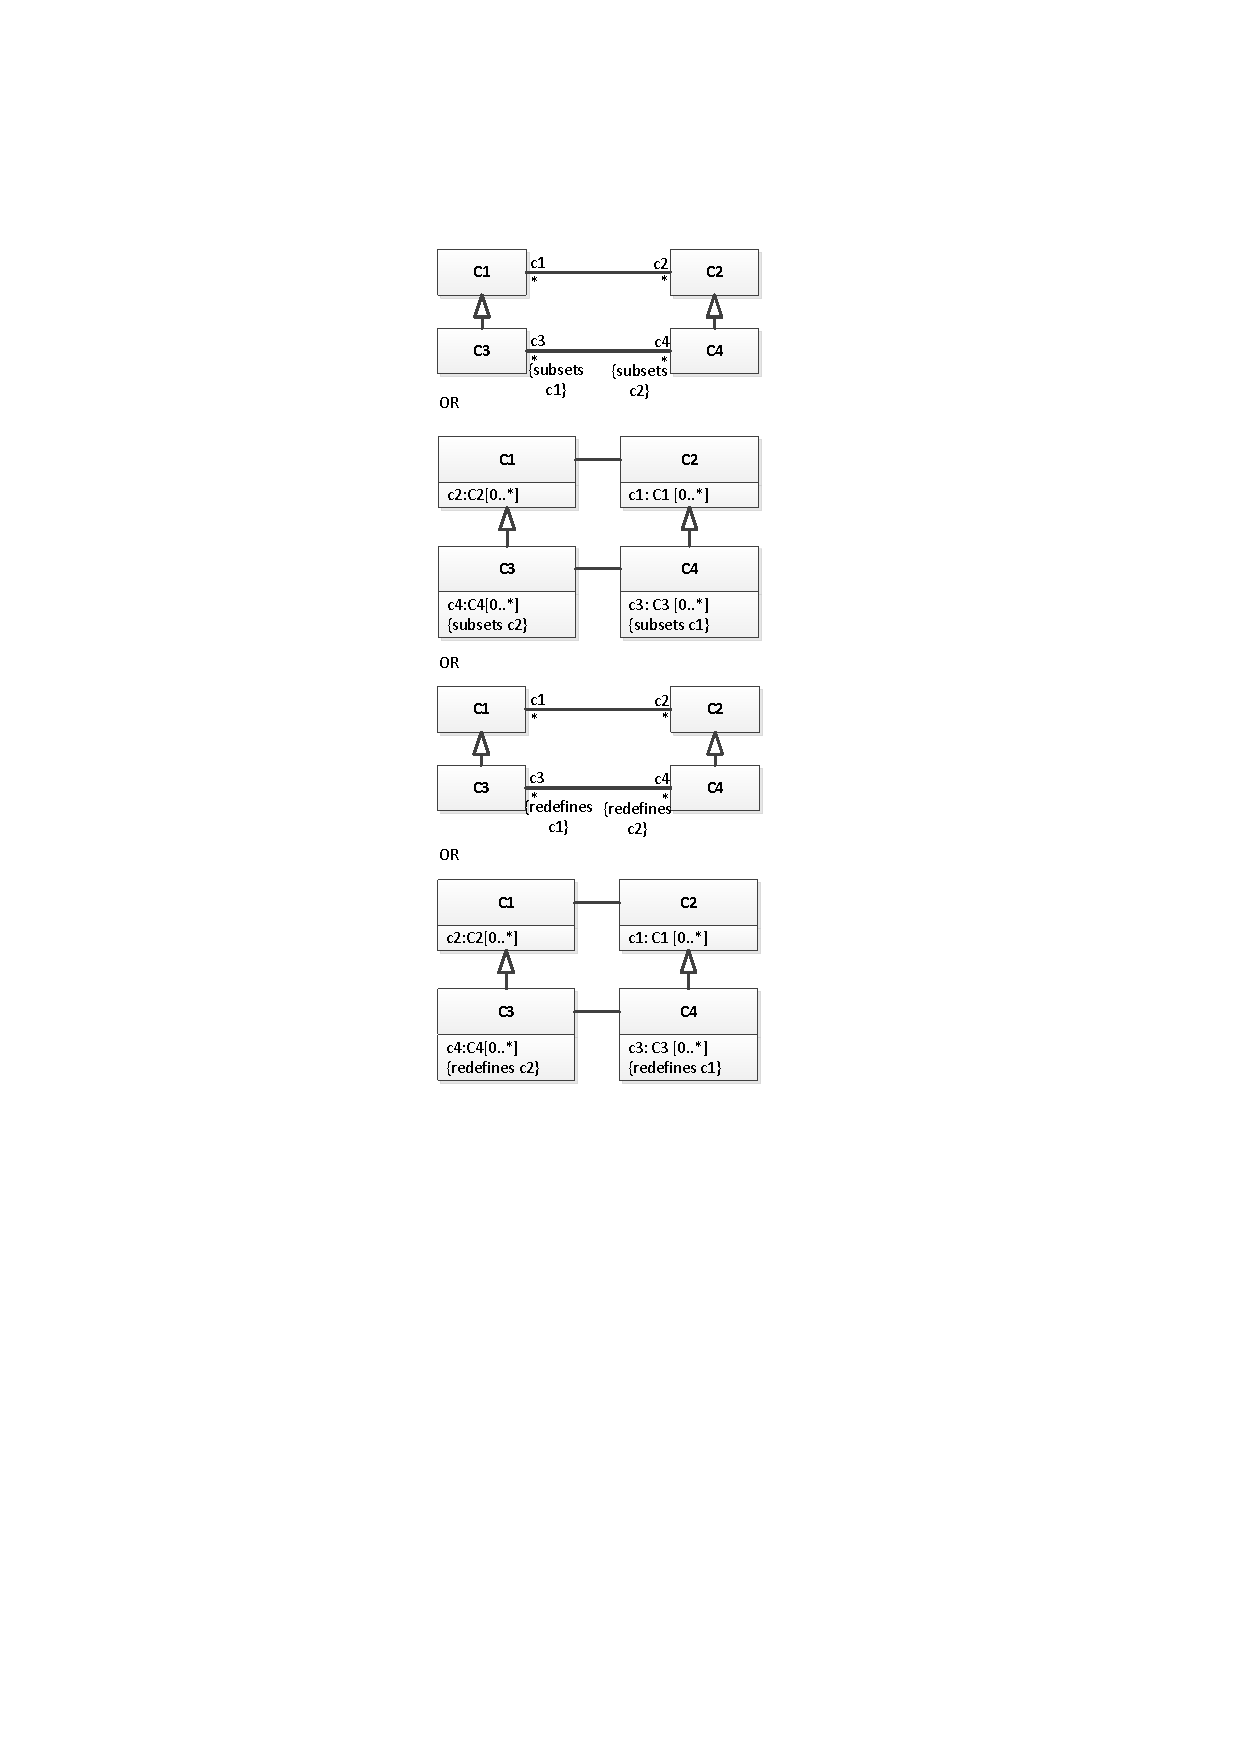
\includegraphics[trim = 72mm 110mm 81mm 35mm, clip, scale=0.75]{./diagrams/chapter5/AssociationAttributeSpecialization}
      Association end (resp. attribute) \texttt{c3} subsets association end (resp. attribute) \texttt{c1} and association end (resp. attribute) \texttt{c4} subsets association end (resp. attribute) \texttt{c2}
      \\OR\\
      Association end (resp. attribute) \texttt{c3} redefines association end (resp. attribute) \texttt{c1} and association end (resp. attribute) \texttt{c4} redefines association end (resp. attribute) \texttt{c2}      
     \vspace{2mm}
    \end{minipage}
    &
    \begin{minipage}{\dltablespacing}
       $\begin{aligned}    	  
    	c_1 &\equiv c_2^-\\ 
    	\exists c_1.\top &\sqsubseteq C_1\\
    	\exists c_1^-.\top &\sqsubseteq C_2\\
    	c_3 &\equiv c_4^-\\
    	\exists c_3.\top &\sqsubseteq C_3\\
    	\exists c_3^-.\top &\sqsubseteq C_4\\    	
    	c_3 &\sqsubseteq c_1\\
    	c_4 &\sqsubseteq c_2  
         \end{aligned}$      
    \end{minipage}
    &
      $\begin{aligned}
        \\
        &\texttt{Class: C1}\\[\owlspacing]
        &\texttt{Class: C2}\\[\owlspacing]
        &\texttt{Class: C3}\\[\owlspacing]
        &\texttt{Class: C4}\\[\owlspacing]
   	&\texttt{ObjectProperty: c1}\\[\owlspacing]
   	&\texttt{\hspace*{0.20cm} Domain: C1}\\[\owlspacing]
   	&\texttt{\hspace*{0.20cm} Range: C2}\\[\owlspacing]
   	&\texttt{\hspace*{0.20cm} InverseOf: c2}\\[\owlspacing]
   	&\texttt{ObjectProperty: c2}\\[\owlspacing]
   	&\texttt{ObjectProperty: c3}\\[\owlspacing]
   	&\texttt{\hspace*{0.20cm} Domain: C3}\\[\owlspacing]
   	&\texttt{\hspace*{0.20cm} Range: C4}\\[\owlspacing]
   	&\texttt{\hspace*{0.20cm} InverseOf: c4}\\[\owlspacing] 
    	&\texttt{\hspace*{0.20cm} SubPropertyOf: c1}\\[\owlspacing]
    	&\texttt{ObjectProperty: c4}\\[\owlspacing]
   	\\
     \end{aligned}$       
    \\\hline
    \begin{minipage}{\umltablespacing}
      \centering\hspace*{-4mm}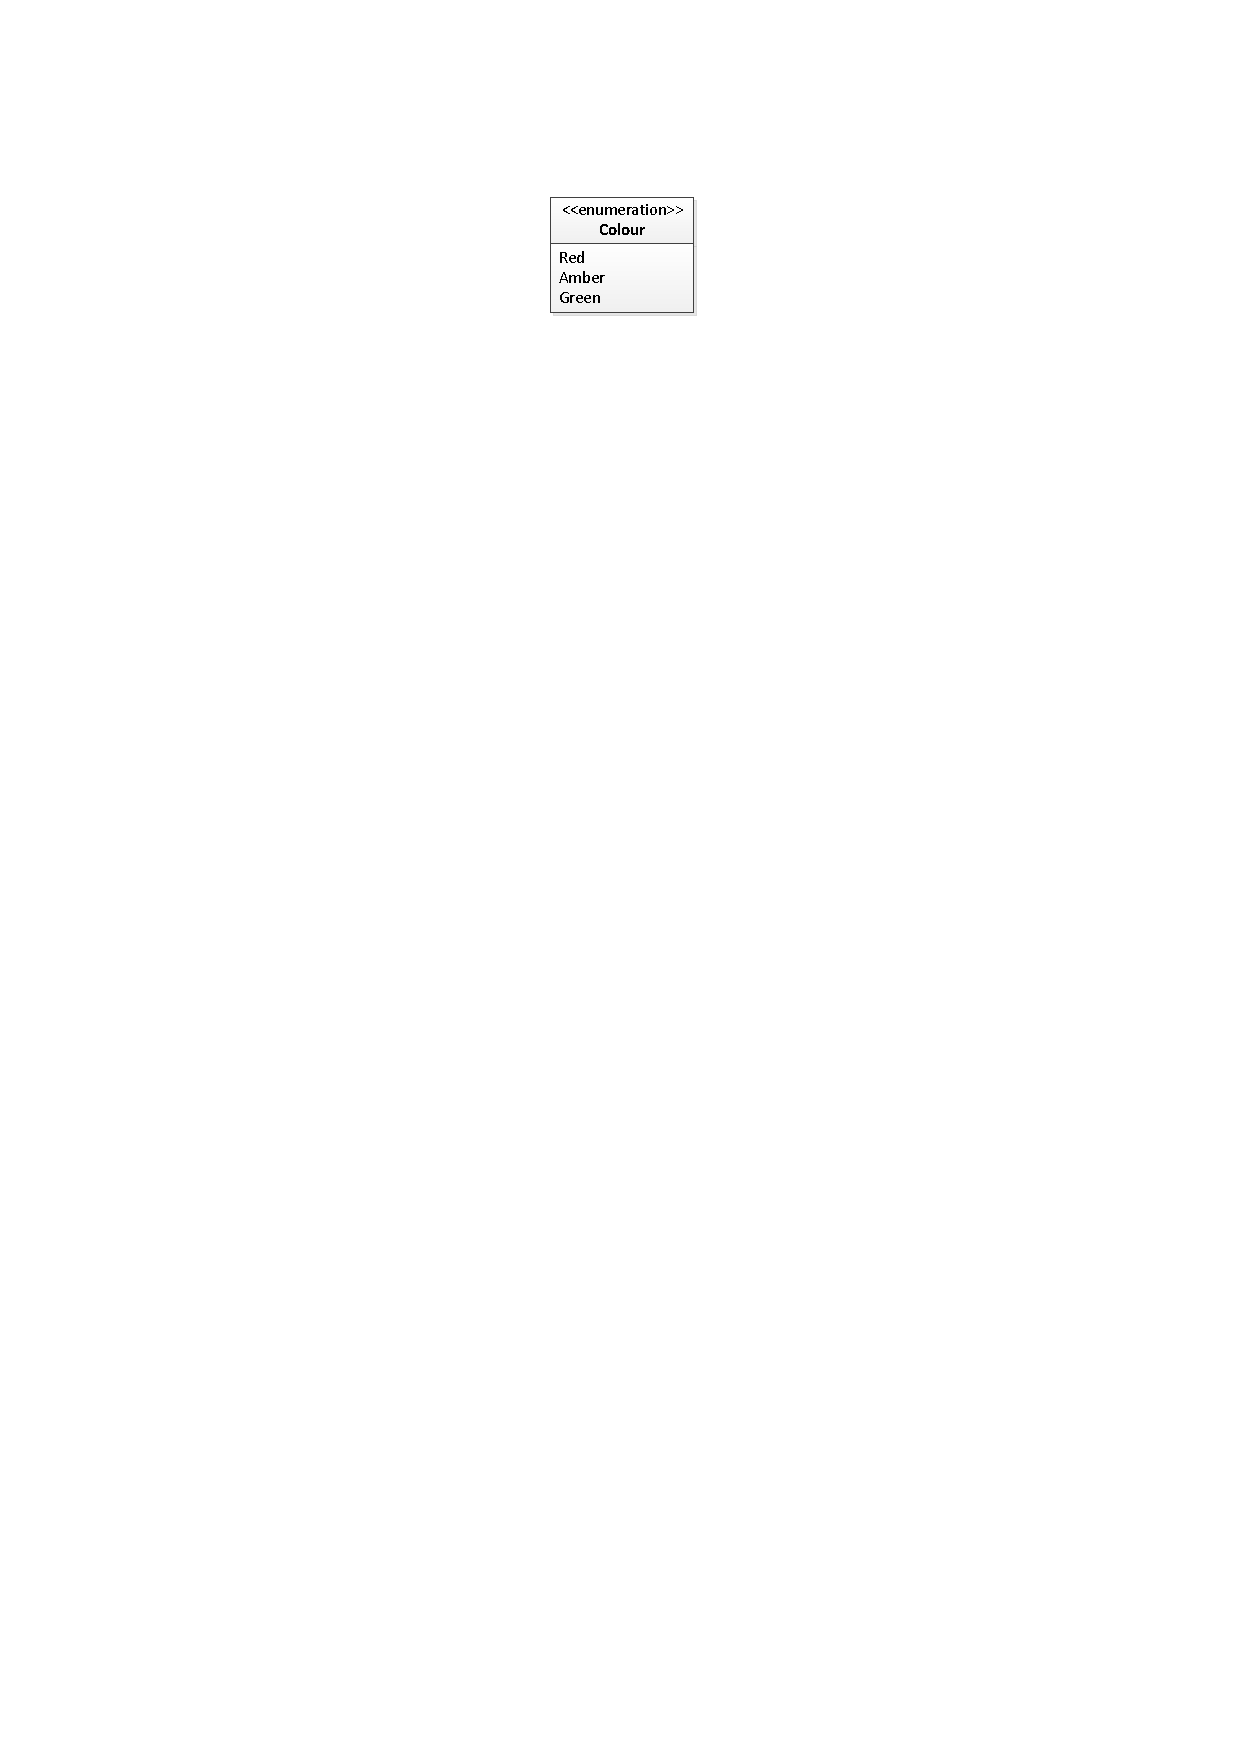
\includegraphics[trim = 80mm 239mm 72mm 25mm, clip, scale=0.75]{./diagrams/chapter5/Enumeration}
      The \texttt{Colour} enumeration consists of the colours \texttt{Red}, \texttt{Amber} and \texttt{Green}
     \vspace{2mm}
    \end{minipage}
    &
    $\begin{aligned}
    Colour &\equiv \{Green, Amber, Red\}\\
    Green &\not\approx Amber\\
    Green &\not\approx Red \\
    Amber &\not\approx Red
    \end{aligned}$
    &
      $\begin{aligned}
      \\
         &\texttt{Class: Colour}\\[\owlspacing]
         &\texttt{\hspace*{2mm} EquivalentTo:}\\[\owlspacing]
         &\texttt{\hspace*{4mm}\{Green, Amber, Red\}}\\[\owlspacing]
         &\texttt{Individual: Green}\\[\owlspacing]
         &\texttt{\hspace*{2mm} Types: Colour}\\[\owlspacing]
         &\texttt{Individual: Amber}\\[\owlspacing]
         &\texttt{\hspace*{2mm} Types: Colour}\\[\owlspacing]
         &\texttt{Individual: Red}\\[\owlspacing]
         &\texttt{\hspace*{2mm} Types: Colour}\\[\owlspacing]
         &\texttt{DifferentIndividuals: }\\[\owlspacing]
         &\texttt{\hspace*{2mm} Green, Amber, Red}\\
     \end{aligned}$    
    \\\hline            
    \begin{minipage}{\umltablespacing}
      \centering\hspace*{-5.5mm}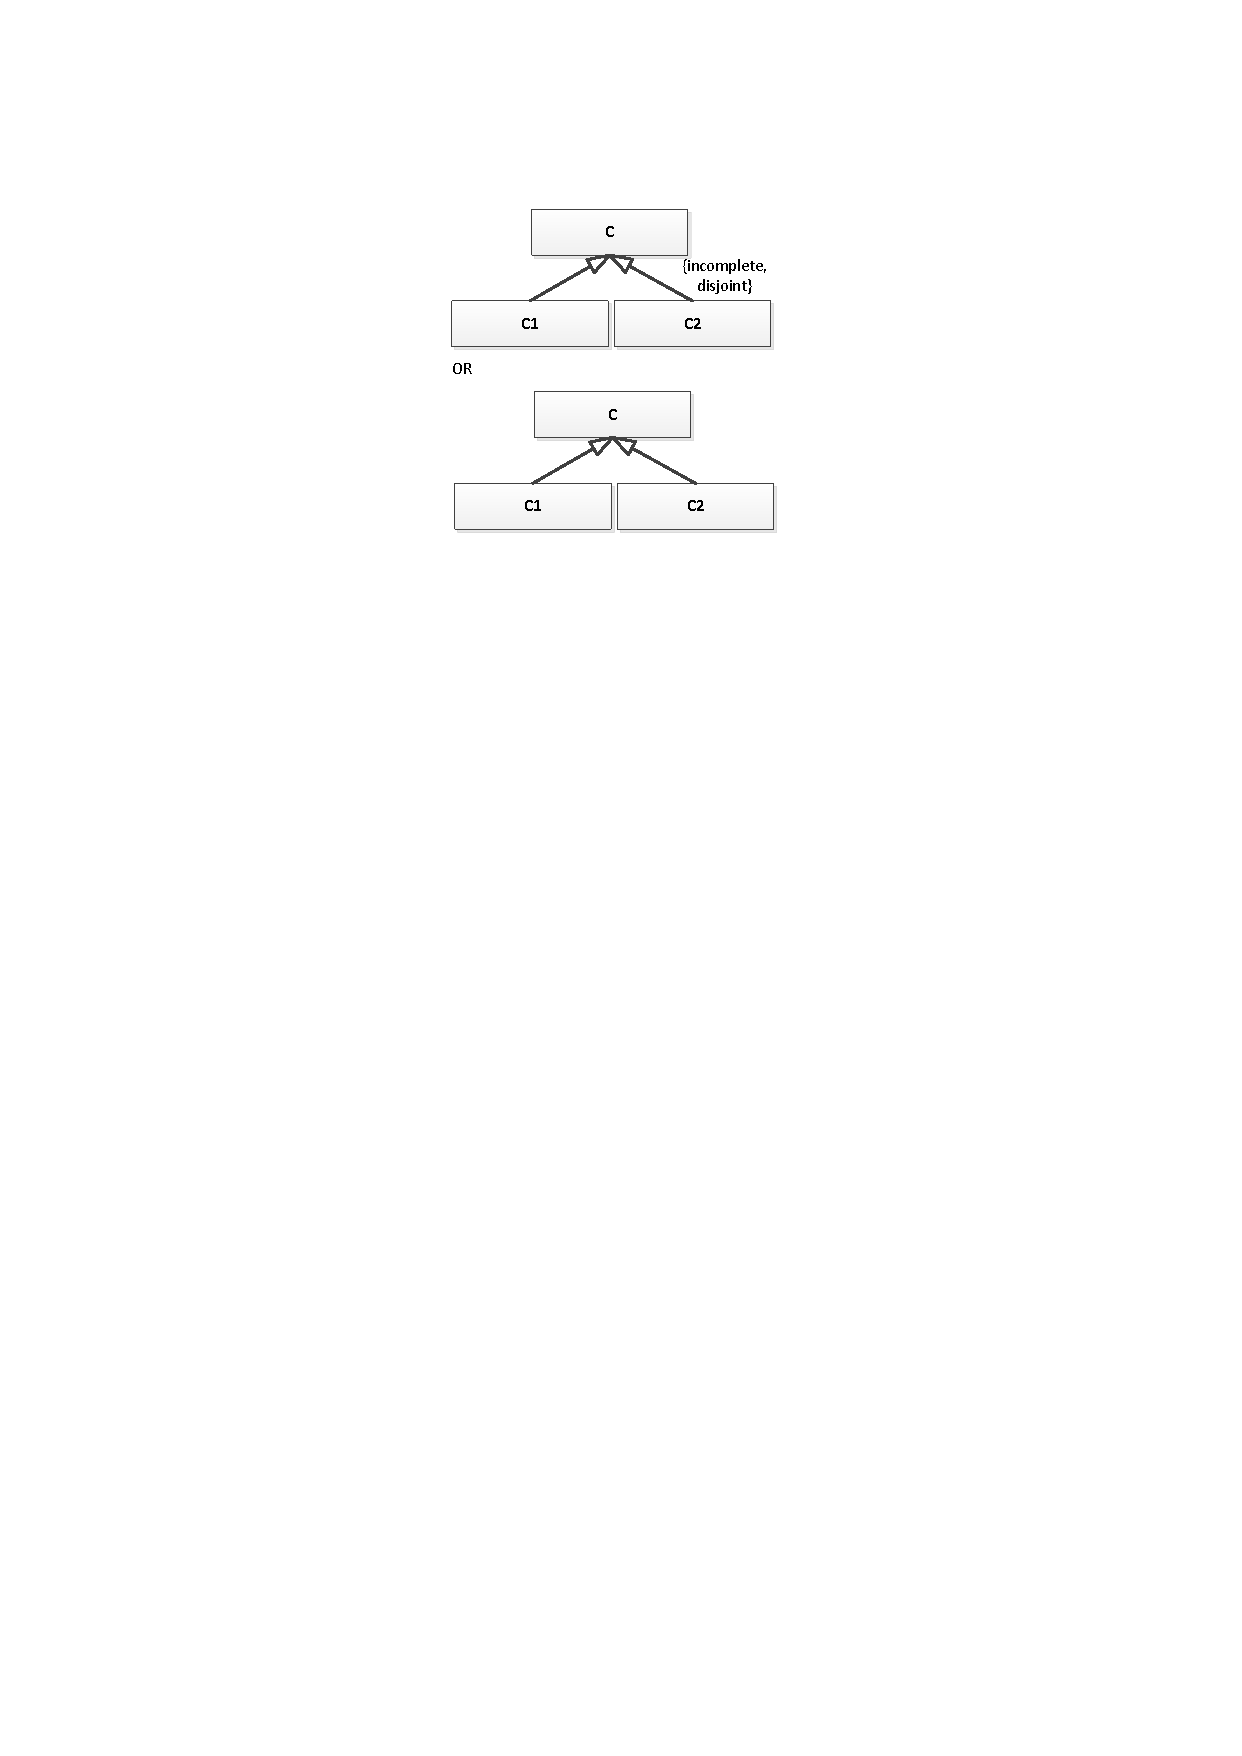
\includegraphics[trim = 76mm 205mm 72mm 25mm, clip, scale=0.75]{./diagrams/chapter5/IncompleteDisjoint}
      Class \texttt{C} is specialized by the disjoint classes \texttt{C1} and \texttt{C2} which do not cover class \texttt{C}
      %Classes \texttt{C1} and \texttt{C2} are disjoint and specialize class \texttt{C} without covering class it 
     \vspace{2mm}
    \end{minipage}
    &
    \begin{minipage}{\dltablespacing}
       $\begin{aligned}    
	  &C_1 \sqsubseteq C  \\  
	  &C_2 \sqsubseteq C \\
	  &C_1 \sqsubseteq \neg C_2
         \end{aligned}$      
    \end{minipage}
    &
      $\begin{aligned}
	  &\texttt{Class: C}\\[\owlspacing]
          &\texttt{Class: C1}\\[\owlspacing]
	  &\texttt{\hspace*{0.20cm}SubClassOf: C}\\[\owlspacing]
          &\texttt{Class: C2}\\[\owlspacing]
          &\texttt{\hspace*{0.20cm}SubClassOf: C}\\[\owlspacing]
          &\texttt{DisjointClasses:}\\[\owlspacing]
          &\texttt{\hspace*{0.20cm}C1, C2}
     \end{aligned}$
     \\\hline
    \begin{minipage}{\umltablespacing}
      \centering\hspace*{-5.5mm}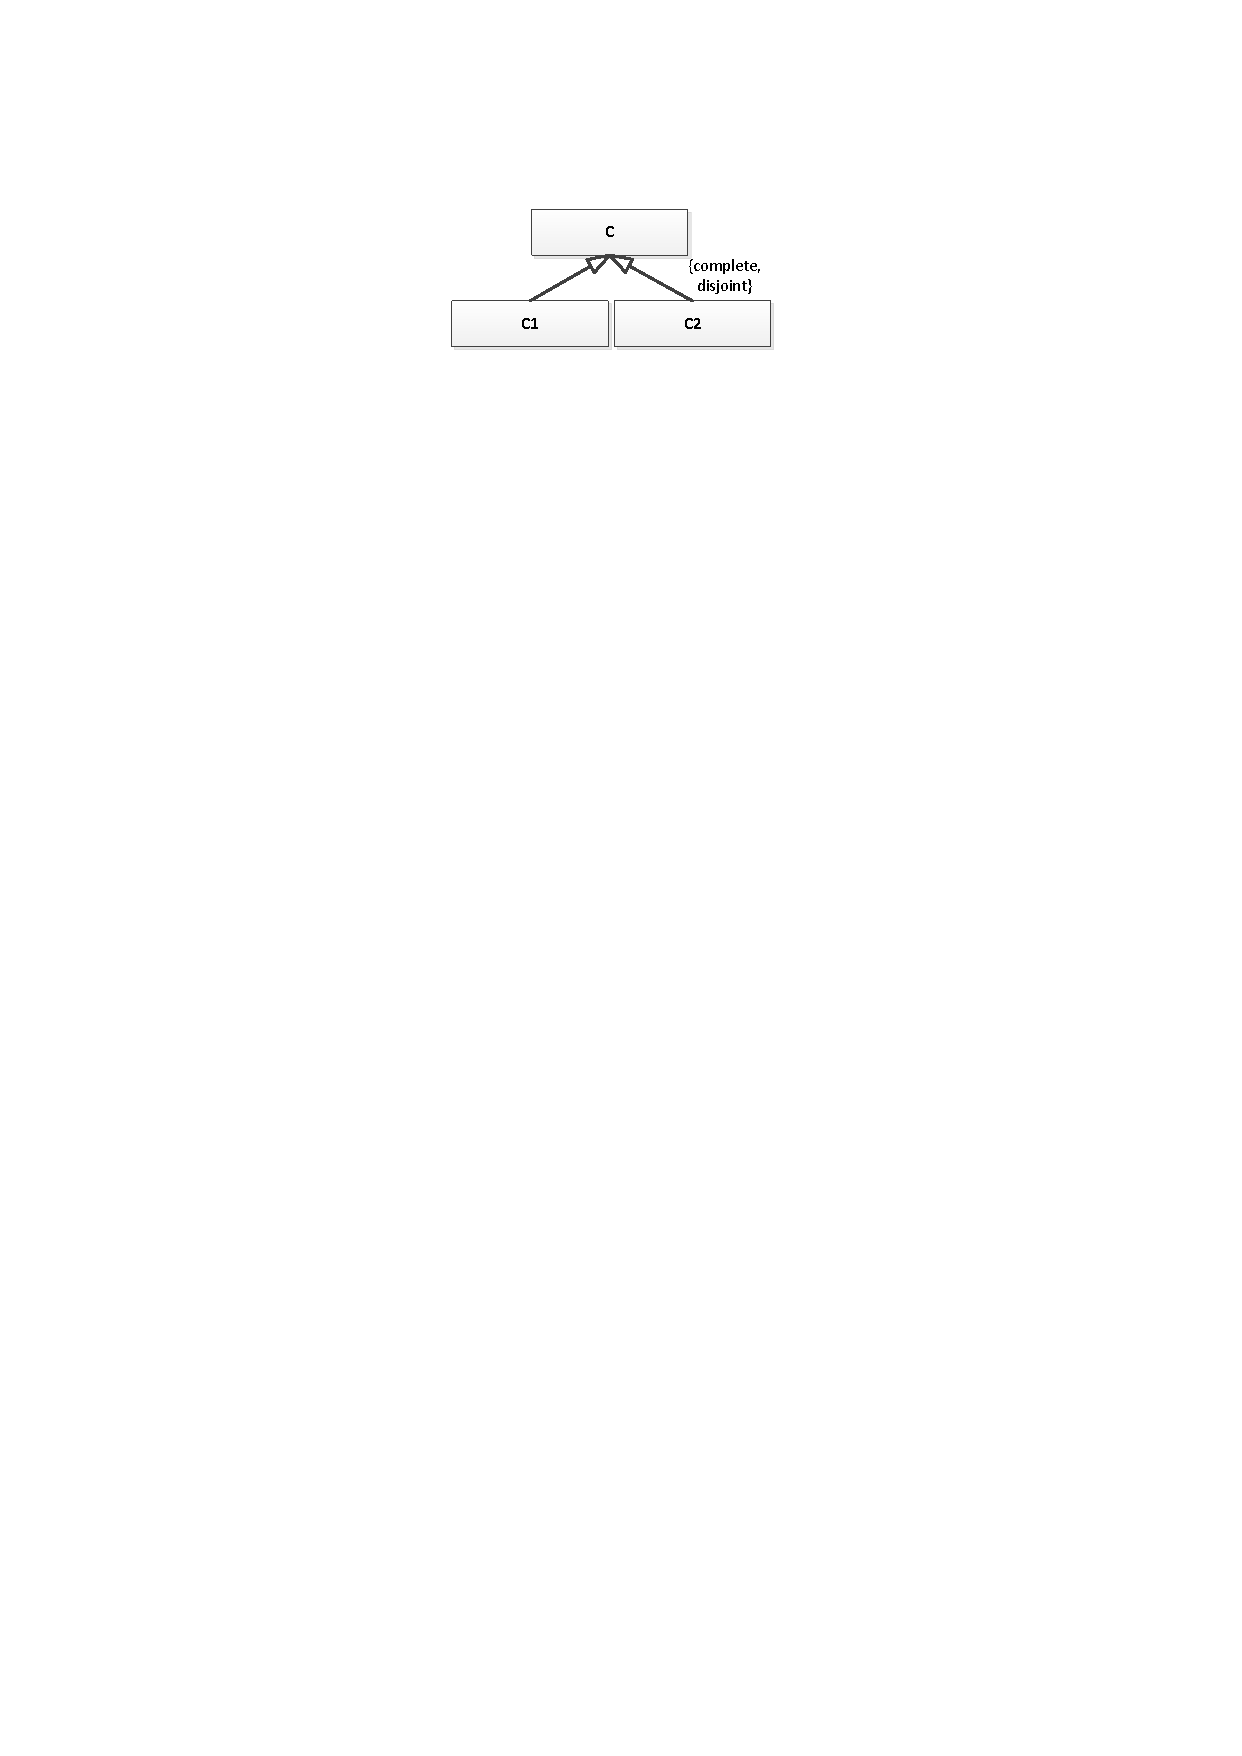
\includegraphics[trim = 76mm 235mm 72mm 25mm, clip, scale=0.75]{./diagrams/chapter5/CompleteDisjoint}
      Class \texttt{C} is specialized by the disjoint classes \texttt{C1} and \texttt{C2} which cover class \texttt{C}  
     \vspace{2mm}
    \end{minipage}
    &
    \begin{minipage}{\dltablespacing}
       $\begin{aligned}   
	  &C \sqsubseteq C_1 \sqcup C_2\\
	  &C_1 \sqsubseteq \neg C_2\\
	  &C_1 \sqsubseteq C  \\  
	  &C_2 \sqsubseteq C 
       \end{aligned}$     
    \end{minipage}
    &
      $\begin{aligned}
	  &\texttt{Class: C}\\[\owlspacing]
	  &\texttt{\hspace*{0.20cm}DisjointUnionOf:}\\[\owlspacing]
	  &\texttt{\hspace*{0.40cm}C1, C2}\\[\owlspacing]
          &\texttt{Class: C1}\\[\owlspacing]
	  &\texttt{\hspace*{0.20cm}SubClassOf: C}\\[\owlspacing]
          &\texttt{Class: C2}\\[\owlspacing]
          &\texttt{\hspace*{0.20cm}SubClassOf: C}	
     \end{aligned}$
     \\\hline     
    \begin{minipage}{\umltablespacing}
      \centering\hspace*{-5.5mm}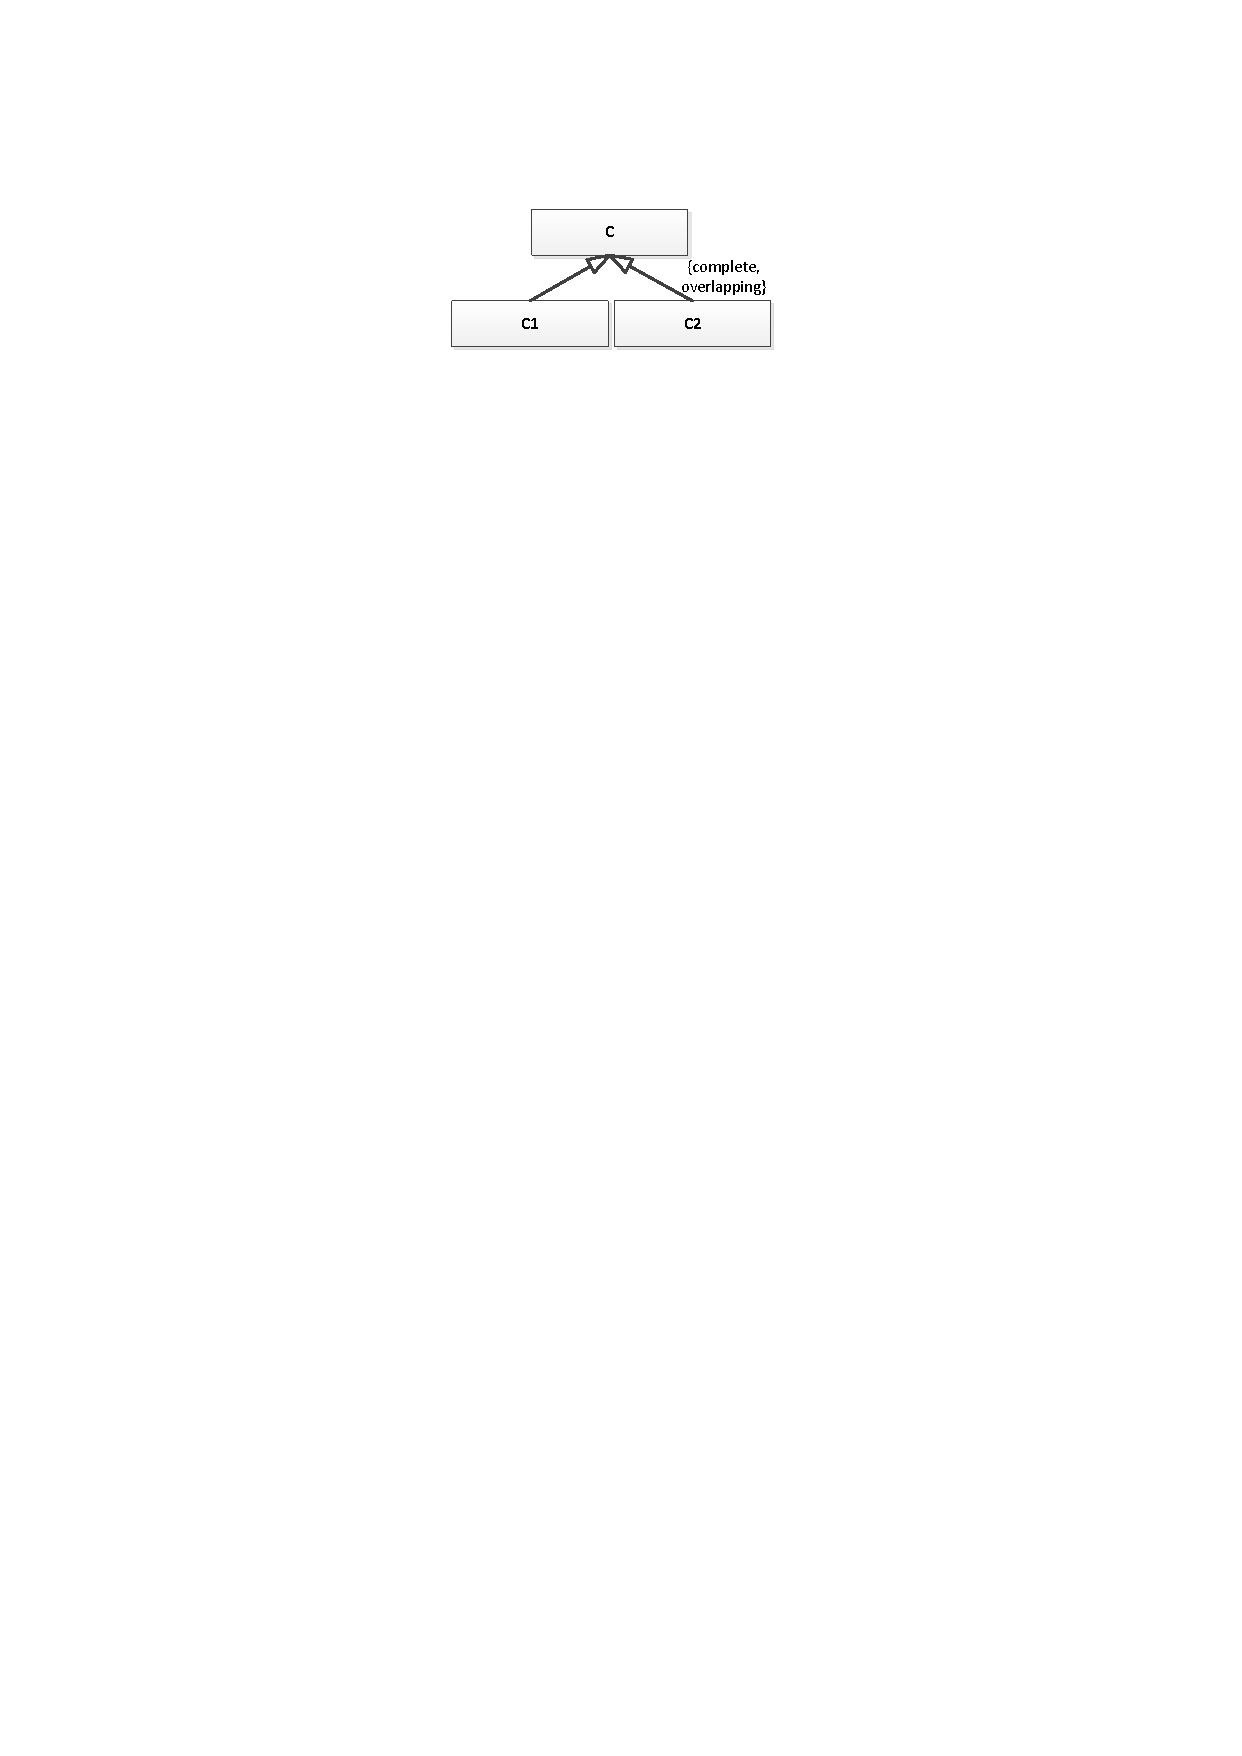
\includegraphics[trim = 76mm 235mm 72mm 25mm, clip, scale=0.75]{./diagrams/chapter5/CompleteOverlapping}
      Class \texttt{C} is specialized by the overlapping classes \texttt{C1} and \texttt{C2} which cover class \texttt{C}  
     \vspace{2mm}
    \end{minipage}
    &
    \begin{minipage}{\dltablespacing}
       $\begin{aligned}   
	  &C \sqsubseteq C_1 \sqcup C_2\\
	  &C_1 \sqsubseteq C  \\  
	  &C_2 \sqsubseteq C 
       \end{aligned}$     
    \end{minipage}
    &
      $\begin{aligned}
	  &\texttt{Class: C}\\[\owlspacing]
	  &\texttt{\hspace*{0.20cm}SubClassOf:}\\[\owlspacing]
	  &\texttt{\hspace*{0.40cm}C1 or C2}\\[\owlspacing]
          &\texttt{Class: C1}\\[\owlspacing]
	  &\texttt{\hspace*{0.20cm}SubClassOf: C}\\[\owlspacing]
          &\texttt{Class: C2}\\[\owlspacing]
          &\texttt{\hspace*{0.20cm}SubClassOf: C}	
     \end{aligned}$
     \\\hline     
    \begin{minipage}{\umltablespacing}
      \centering\hspace*{-5.5mm}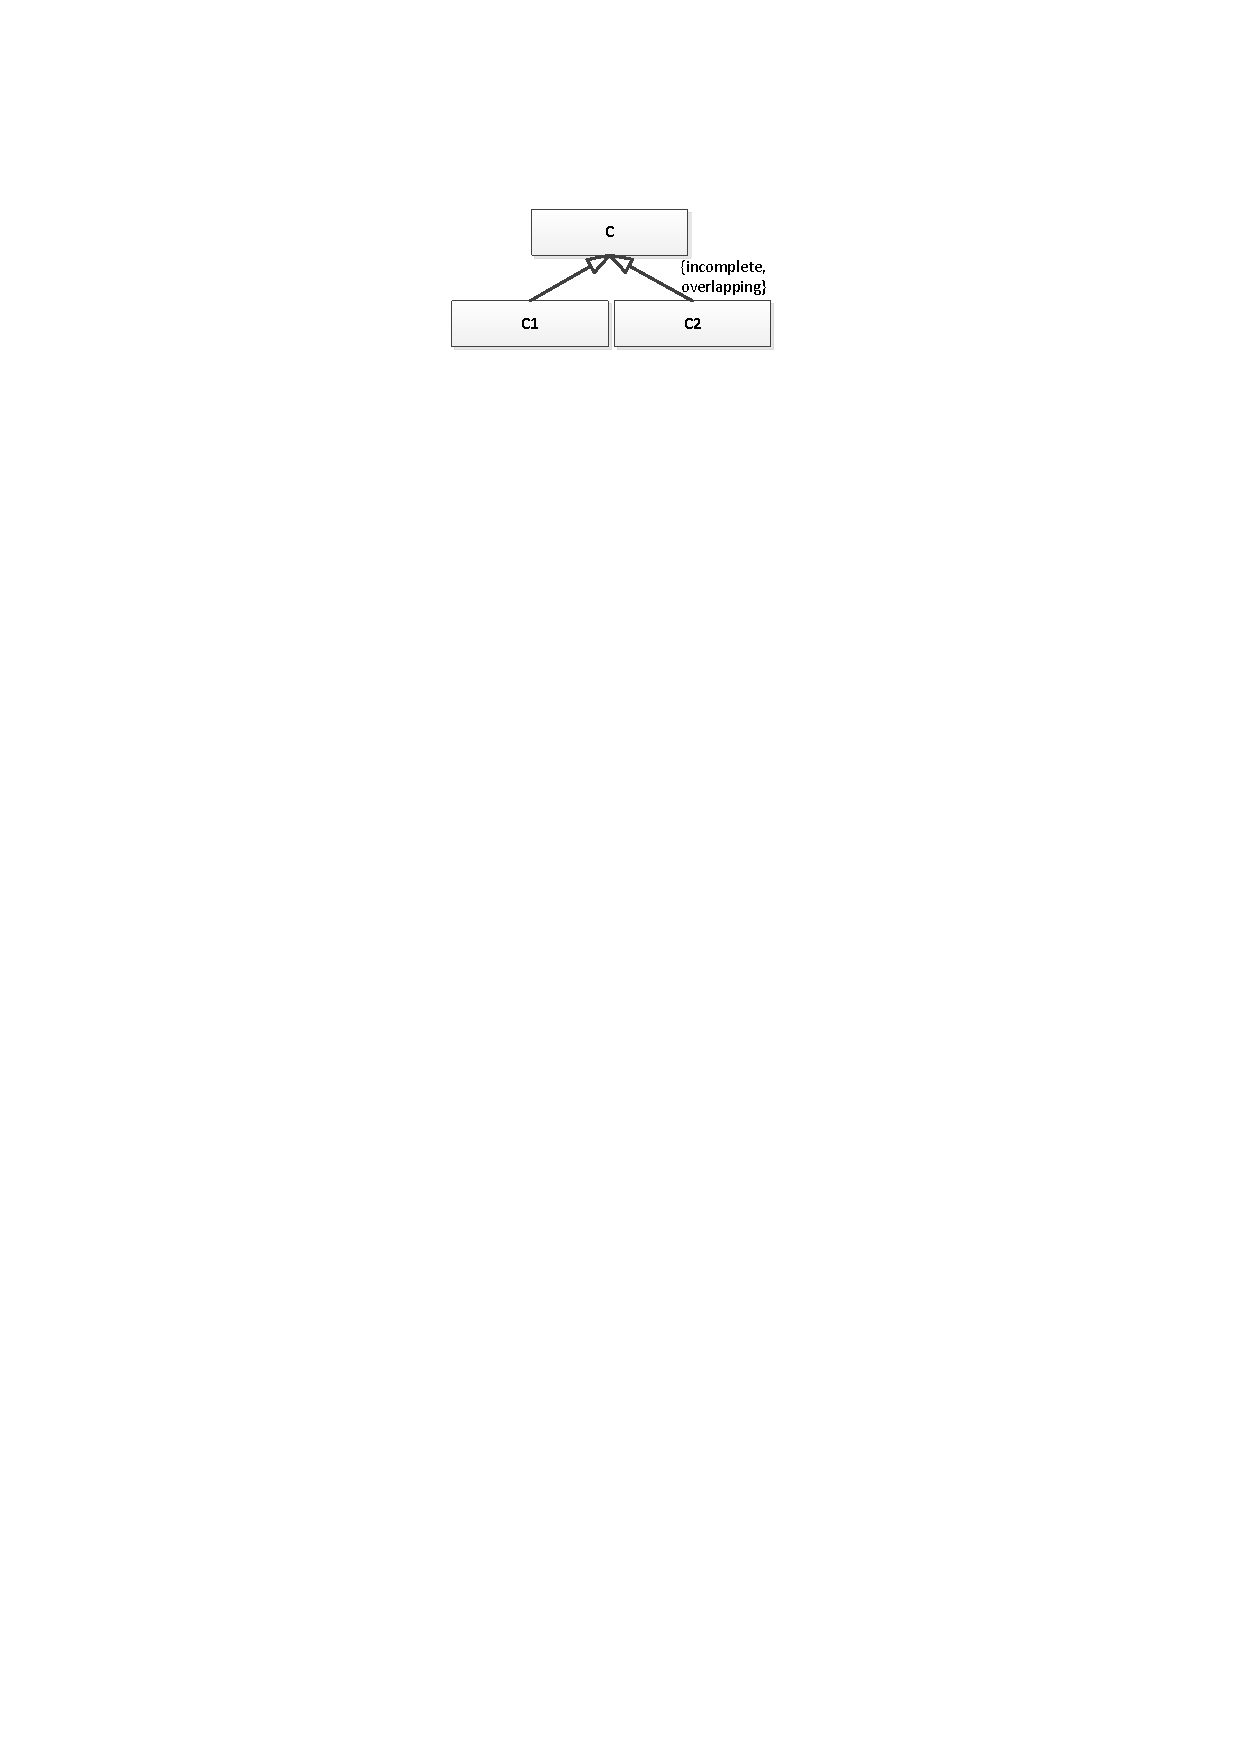
\includegraphics[trim = 76mm 235mm 72mm 25mm, clip, scale=0.75]{./diagrams/chapter5/IncompleteOverlapping}
      Class \texttt{C} is specialized by the overlapping classes \texttt{C1} and \texttt{C2} which do not cover class \texttt{C}  
     \vspace{2mm}
    \end{minipage}
    &
    \begin{minipage}{\dltablespacing}
       $\begin{aligned}   
	  &C_1 \sqsubseteq C  \\  
	  &C_2 \sqsubseteq C 
       \end{aligned}$     
    \end{minipage}
    &
      $\begin{aligned}
	  &\texttt{Class: C}\\[\owlspacing]
          &\texttt{Class: C1}\\[\owlspacing]
	  &\texttt{\hspace*{0.20cm} SubClassOf: C}\\[\owlspacing]
          &\texttt{Class: C2}\\[\owlspacing]
          &\texttt{\hspace*{0.20cm} SubClassOf: C}	
     \end{aligned}$
     \\\hline       
    \begin{minipage}{\umltablespacing}
    %trim option's parameter order: left bottom right top
      \centering\hspace*{-4.7mm}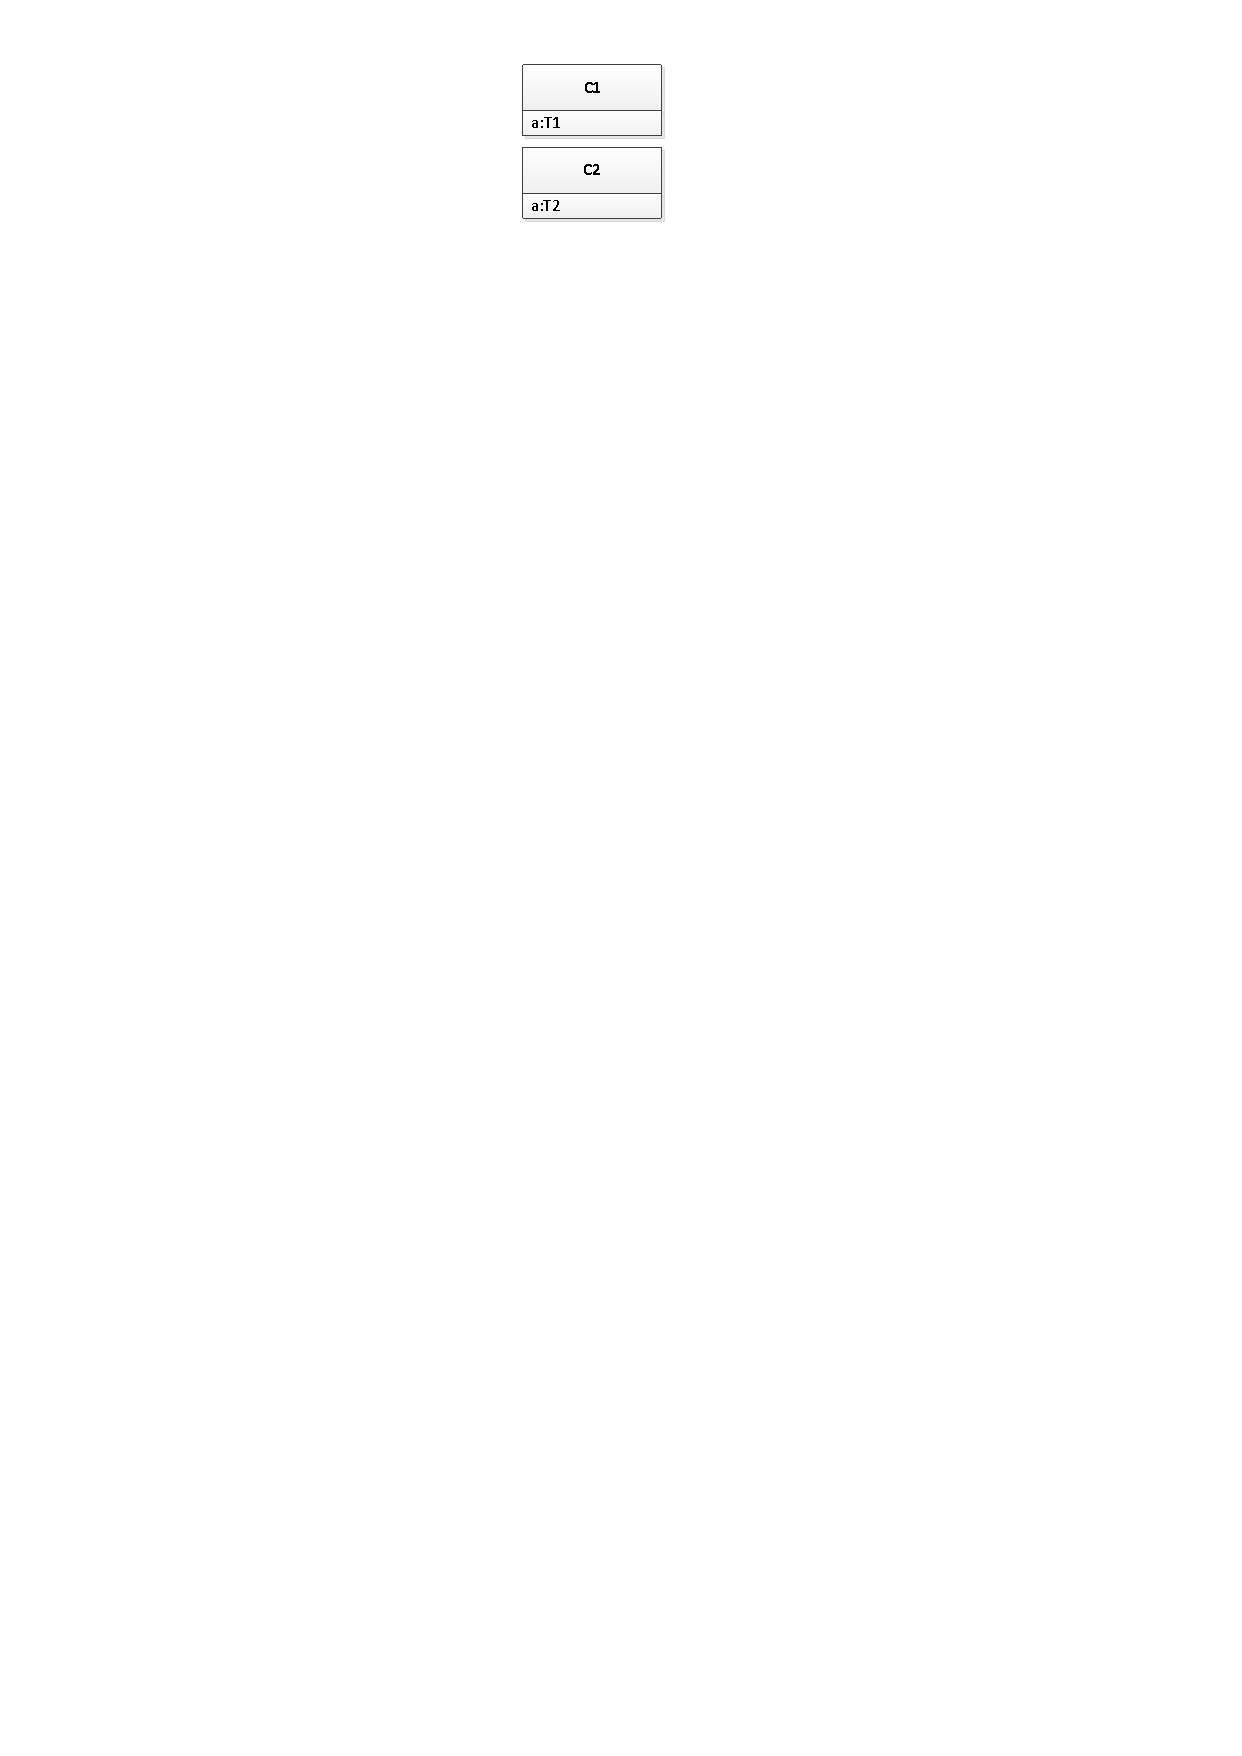
\includegraphics[trim = 76mm 255mm 72mm 0mm, clip, scale=0.75]{./diagrams/chapter5/QualifiedAttributeNamesSmall}
      Classes \texttt{C1} and \texttt{C2} both have an attribute \texttt{a} respectively of type \texttt{T1} and \texttt{T2}.
     \vspace{2mm}
    \end{minipage}
    &
    \begin{minipage}{\dltablespacing}
    $\begin{aligned}
  	&\exists a.\top \sqsubseteq C_1 \sqcup C_2\\
  	&\exists a^-.\top \sqsubseteq T_1 \sqcup T_2\\
  	&C_1 \sqsubseteq \exists a.\top \sqcap (\leq 1 \hspace*{2pt} a. \top)\\
  	&C_2 \sqsubseteq \exists a.\top \sqcap (\leq 1 \hspace*{2pt} a. \top)
    \end{aligned}$
    \end{minipage}
    &
     $\begin{aligned} 
	&\texttt{Class: C1} \\[\owlspacing]
   	&\texttt{\hspace*{2mm}SubClassOf:}\\[\owlspacing]
   	&\texttt{\hspace*{4mm}t exactly 1 Thing}\\[\owlspacing]	
	&\texttt{Class: C2} \\[\owlspacing]
   	&\texttt{\hspace*{2mm}SubClassOf:}\\[\owlspacing]
   	&\texttt{\hspace*{4mm}t exactly 1 Thing}\\[\owlspacing]	
	&\texttt{Class: T1} \\[\owlspacing]
	&\texttt{Class: T2} \\[\owlspacing]	
	&\texttt{ObjectProperty: a} \\[\owlspacing]
	&\texttt{\hspace*{2mm} Domain: C1 or C2} \\[\owlspacing]
	&\texttt{\hspace*{2mm} Range: T1 or T2} \\
    \end{aligned}$     
     \\\hline 
    \end{longtable} 
 
\end{document}
